% This is a LaTeX thesis template for Monash University.
% to be used with Rmarkdown
% This template was produced by Rob Hyndman
% Version: 6 September 2016

\documentclass{monashthesis}

%%%%%%%%%%%%%%%%%%%%%%%%%%%%%%%%%%%%%%%%%%%%%%%%%%%%%%%%%%%%%%%
% Add any LaTeX packages and other preamble here if required
%%%%%%%%%%%%%%%%%%%%%%%%%%%%%%%%%%%%%%%%%%%%%%%%%%%%%%%%%%%%%%%

\author{Huize Zhang}
\title{Exploration of Judicial Facial Expression in Videos of Legal Proceedings}
\studentid{27478343}
\def\degreetitle{Bachelor of Commerce (Honours)}
% Add subject and keywords below
\hypersetup{
     %pdfsubject={The Subject},
     %pdfkeywords={Some Keywords},
     pdfauthor={Huize Zhang},
     pdftitle={Exploration of Judicial Facial Expression in Videos of Legal Proceedings},
     pdfproducer={Bookdown with LaTeX}
}


\bibliography{thesisrefs}

\begin{document}

\pagenumbering{roman}

\titlepage

{\setstretch{1.2}\sf\tighttoc\doublespacing}

\clearpage\pagenumbering{arabic}\setcounter{page}{0}

\hypertarget{acknowledgements}{%
\chapter*{Acknowledgements}\label{acknowledgements}}
\addcontentsline{toc}{chapter}{Acknowledgements}

I would like to express my gratitude to Professor Di Cook, my supervisors, for detailed guidance and kindness support thorughout and Professor Russell Smyth for raising the idea of this project. I would like to appreciate Stephanie Kobakian, with whom I have countless discussion with about the project. I would also like to extend my thank to my friends, colleages and family for standing behind me unconditionally.

\hypertarget{declaration}{%
\chapter*{Declaration}\label{declaration}}
\addcontentsline{toc}{chapter}{Declaration}

I hereby declare that this thesis contains no material which has been accepted for the award of any other degree or diploma in any university or equivalent institution, and that, to the best of my knowledge and belief, this thesis contains no material previously published or written by another person, except where due reference is made in the text of the thesis.

\vspace*{2cm}\par\authorname

\hypertarget{abstract}{%
\chapter*{Abstract}\label{abstract}}
\addcontentsline{toc}{chapter}{Abstract}

It is part of the human nature to express emotions as a way to react. However, in particular situation, for example the court, the Justices need to restrict their emotions display as a requirement to ensure the judgement is not biased towards a particular party. In this study, we use facial recognition software to objectively assess the facial expressions of six Justices in seven cases from the high court of Australia. From the obtained facial variables, we model the presence of a selected range of action units by a binomial model and the intensity of the action units by a two part model. From the modelling, we observe that the Justices are remain impartial during the court in general. When a more intense or frequent action unit is presented, it tends to be associated with a negative emotion like sad, fear and anger. Also we find that it would be hard for some Justices to remain a still face in the criminal cases where more extreme behaviour like drug issue and sexual assult are involved.

\clearpage\pagenumbering{arabic}\setcounter{page}{1}

\hypertarget{ch:intro}{%
\chapter{Introduction}\label{ch:intro}}

\hypertarget{background-and-motivation}{%
\section{Background and motivation}\label{background-and-motivation}}

People have attempted to predict the decisions of the Justices in the past century using judge characteristics i.e.~Gender, political views, religious background. More recently, scholars\autocites{Shullman2004illusion}{chen2018justice} have been using more information from media(i.e.~AV recording, transcript, language used by the Justices) to predict the case outcome using the U.S. Supreme Court data. On-court information has also been used to study data from High Court of Australia. \textcite{tutton2018judicial} has used an ethnographic approach to present a observational study of judicial behaviour based on watching the audio footage. Manually observing the AV recordings could lead to subjective evaluation of facial expression and this motivates us \emph{to build upon \textcite{tutton2018judicial}'s work to employ facial recognition technology to study the facial expression of the justices, which will provide a more objective result than \textcite{tutton2018judicial}}.

\hypertarget{literature-review}{%
\section{Literature review}\label{literature-review}}

The literature summary is divided into two parts: (1) current work in legal studies to understand the behaviour of the Justices and (2) existing facial recognition and emotion tagging technology.

\hypertarget{legal-study-from-a-behaviour-perspective}{%
\subsection{Legal study from a behaviour perspective}\label{legal-study-from-a-behaviour-perspective}}

There is a large law \& economics and political science literature that attempts to predict how judges will vote in court cases. Much of this focuses on the characteristics of the judge i.e.~gender, political views, religious background and characteristics of the parties in the case i.e.~gender or race of the defendant in criminal cases \autocites{Stuart1962}{Peter1984}{Combining1987}{Susan1988}{Steffensmeier2001}{Kulik2003}.

Moving from static information of the judge and parties involved, more studies start to incorporate the language used by the judge on the court to predict the decision of the Justices. \textcite{black2011emotions} has study the use of pleasant and unpleasant language by the Justices and \textcite{Shullman2004illusion} and \textcite{johnson2009inquiring} have studied the effect of frequency and content of Justices' questions. \textcite{epstein2010inferring} use a regression analysis with the number of questions asked by the Justices used to infer the winning party in a case.

More recent legal study has focused on the usage of emotion and vocal characteristics of the Justices to predict the judge's votes. Although \textcite{judicalguid} present the following code of conduct:

\begin{quote}
It is important for judges to maintain a standard of behaviour in court that is consistent with the status of judicial office and does not diminish the confidence of litigants in particular, and the public in general, in the ability, the integrity, the impartiality and the independence of the judge.
\end{quote}

and this impartiality has been highlighted in judicial demeanour by \textcite{tutton2018judicial} and \textcite{goffman1956nature}, Paul Ekman \textcite{ekman1991invited} suggests that from a behavioural perspective, some facial and vocal inflections are often unbeknown to the speakers themselves. \textcite{chen2016perceived}; \textcite{chen2017covering} and \textcite{schubert1992observing} have studied the emotion of the Justices from vocal characteristics and suggest that these vocal characteristics, especially perceived masculinity is strongly correlated with the court outcomes. \textcite{dietrich2019emotional} has used a multilevel logistic model with random effects to suggest that subconscious vocal inflections contain information that is not available from text.

Moreover, a more sizeable study by \textcite{chen2018justice} have incorporated both vocal and image information of the judge into a machine learning model to predict the judge votes and case outcome using the U.S. Supreme Court data from 1946-2014. He found that image features improved prediction of case outcomes from 64\% to 69\% and audio features improved prediction of case outcomes from 67\% to 69\%. This demonstrates the potential of incorporating facial information to understand the decision of the Justices.

The literature mentioned above is mostly conducted using the U.S. Supreme Court Database and less studies have been conducted using Australian High Court data. \textcite{tutton2018judicial} has used an ethnographic approach to study the judicial demeanour in the High Court of Australia and it is the first of its kind to use transcript and AV recordings in Australian study. The study found that Justices present a detached facial demeanour during the court in most of the time while some human display of emotions i.e.~laughter and humour have also been captured by the scholars. Tutton's work has confirmed the potential of using image information to understanding the Justices as in Chen's study, while the ethnographic approach could be biased and lead to subjective results when different people are observing the videos. Thus, building upon Tutton's study, my work fills the gap of producing objective result via utilising facial recognition technology.

\hypertarget{facial-recognition}{%
\subsection{Facial recognition}\label{facial-recognition}}

An anatomical study of the decomposition of facial muscles by \autocite{ekman1976measuring} led to the development of Facial Action Code (FAC) \autocite{ekman1978} and identification of the six universal emotions on human faces. This work has laid a solid foundation for analysing facial expression and developing facial recognition software for researchers \autocites{Kobayashi1992}{huang1997}{lien2000}{Kappoor2003}{Tong2007}{Cohn2009}{Lucey2010}.

To be able to analysis the facial expression, proper facial recognition technique is needed to first extract faces from images. Facial recognition software i.e.~DeepFace \autocite{taigman2014deepface} from Facebook and FaceNet \autocite{schroff2015facenet} from Google have also been developed for face detection. OpenFace \autocite{baltrusaitis2018openface} is the first open-sourced face recognition software that provides facial expression detection, including facial landmarking, head pose estimation, eye gaze tracking and facial action unit detection. The OpenFace toolkit has been used in different area in research including depression classification \autocites{yang2016decision}{nasir2016multimodal}, emotion study \autocites{Pan2018}{Nasir2016}{Huber2018} and even sports analytics. \autocite{kovalchik2018going}.

\hypertarget{data-collection}{%
\chapter{Data Collection}\label{data-collection}}

\hypertarget{data-processing}{%
\section{Data Processing}\label{data-processing}}

The source data of this research project is the AV recordings publicly available from the High Court of Australia \autocite{highcourtau}. Due to the requirement of resolution (more than 30px for face detection) of OpenFace, we picked up seven cases from 2018 that have less than seven judges as the sample videos for our dataset. A full list of video being processed can be found in Table \ref{tab:case-info} in the Appendix.

Multiple procedures need to be performed to obtain the numerical value of facial variables from the source videos. The entire workflow has been plotted in Figure \ref{fig:workflow}. Youtube-dl \autocite{youtube-dl} has been used to download videos from the High Court of Australia \autocite{highcourtau}. Image frames are extracted from the videos for every minute via ffmpeg \autocite{ffmpeg}, resulting in 1021 image frames. Because the Justices are remain seated at the same position throughout the hearing, Taipan \autocite{Taipan} is used to find the x-y coordinates of the location of the Justices in each image frame. ImageMagick \autocite{ImageMagick} is followed to crop the face of each Justice from each image frame based on the coordinates from Taipan. The resulting 4601 cropped faces are then sent to OpenFace \autocite{baltrusaitis2018openface} to process on Docker. The output of OpenFace contains facial variables like facial landmarking, head pose, eye gaze and action unit. These outputs are stored as separate comma-separated values (csv) files for each of the 4601 faces and post-processing is done in R to combine all the separate csv files into a final dataframe with appropriate index of frame, judge and video added.

\begin{figure}

{\centering 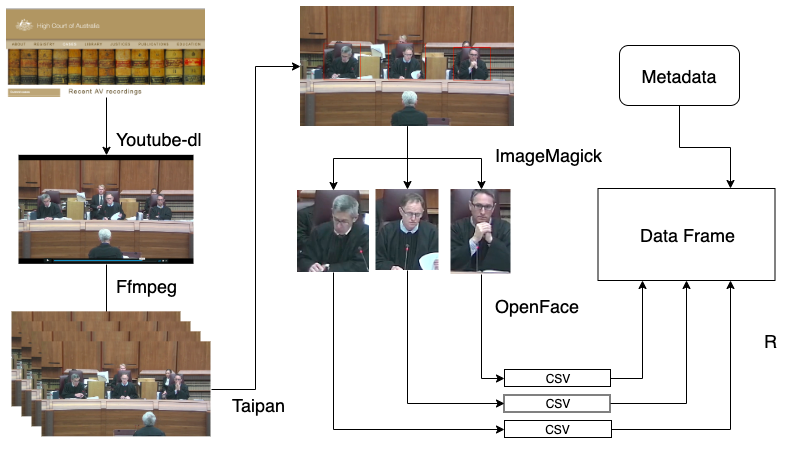
\includegraphics[width=1\linewidth]{figures/workflow} 

}

\caption{This is an illustration of the workflow for extracting facial variables from videos. \label{fig:workflow}}\label{fig:unnamed-chunk-1}
\end{figure}

\hypertarget{variable-description}{%
\section{Variable description}\label{variable-description}}

OpenFace provides more than 711 variables measuring different aspects of a given face and a full description of the output variables can be found in \textcite{baltrusaitis2018openface}. The facial variables can be summarised into the following categories.

\begin{itemize}
\item
  \textbf{Confidence}: How confidence OpenFace is with the detection. Confidence is related to the angle that the Justice's face present in the images.
\item
  \textbf{Gaze}: Gaze tracking: the vector from the pupil to corneal reflection. The dataset contains information on the gaze for both eyes while there is no distinct difference between the eyes. Also I was trying to make animation to track the change of the gaze for judges but no good luck.
\item
  \textbf{Pose}: the location of the head with respect to camera. Pose-related variables don't provide much useful information apart from gaze-related variables.
\item
  \textbf{Landmarking}: landmarking variables for face and eyes. Landmarking variables allows me to plot the face of the judge in a particular frame. More work could be done to explore the usefulness of landmarking variables.
\item
  \textbf{Action Unit}: Action units are used to describe facial expressions. The action unit has intensity measures ending with \texttt{\_c} and presence measures ending with \texttt{\_r}.
\end{itemize}

In this project, we will focus on using action units along with information about judge, video, speaker to analyse the face of the judge.

\hypertarget{data-format}{%
\section{Data format}\label{data-format}}

The data can be expressed in the long format with action unit being an index and presence and intensity being two columns. The Table \ref{tab:long} presents the data for Justices Edelman in video McKell for all the action unit in the first frame in long format. Figure \ref{fig:ts-plot} plots the presence and intensity across time.

\begin{table}[ht]
\begin{center}
\caption{\label{tab:long} This table is an illustration of a proportion of the data in long format.}
\begin{tabular}{lllllll}
\toprule
judge & video & frame & speaker & AU & presence & intensity \\
\midrule
Edelman & McKell & 1 & Appellent & AU01 & 0 & 0.05 \\
Edelman & McKell & 1 & Appellent & AU02 & 0 & 0.00 \\
Edelman & McKell & 1 & Appellent & AU04 & 0 & 0.01 \\
Edelman & McKell & 1 & Appellent & AU05 & 0 & 0.00 \\
Edelman & McKell & 1 & Appellent & AU06 & 0 & 0.00 \\
Edelman & McKell & 1 & Appellent & AU07 & 0 & 0.00 \\
Edelman & McKell & 1 & Appellent & AU09 & 0 & 0.26 \\
Edelman & McKell & 1 & Appellent & AU10 & 0 & 0.00 \\
Edelman & McKell & 1 & Appellent & AU12 & 0 & 0.00 \\
Edelman & McKell & 1 & Appellent & AU14 & 1 & 1.23 \\
Edelman & McKell & 1 & Appellent & AU15 & 0 & 0.46 \\
Edelman & McKell & 1 & Appellent & AU17 & 0 & 0.66 \\
Edelman & McKell & 1 & Appellent & AU20 & 1 & 1.44 \\
Edelman & McKell & 1 & Appellent & AU23 & 0 & 0.64 \\
Edelman & McKell & 1 & Appellent & AU25 & 0 & 0.00 \\
Edelman & McKell & 1 & Appellent & AU26 & 0 & 0.00 \\
Edelman & McKell & 1 & Appellent & AU45 & 0 & 0.25 \\
\bottomrule
\end{tabular}
\end{center}
\end{table}

\begin{figure}

{\centering 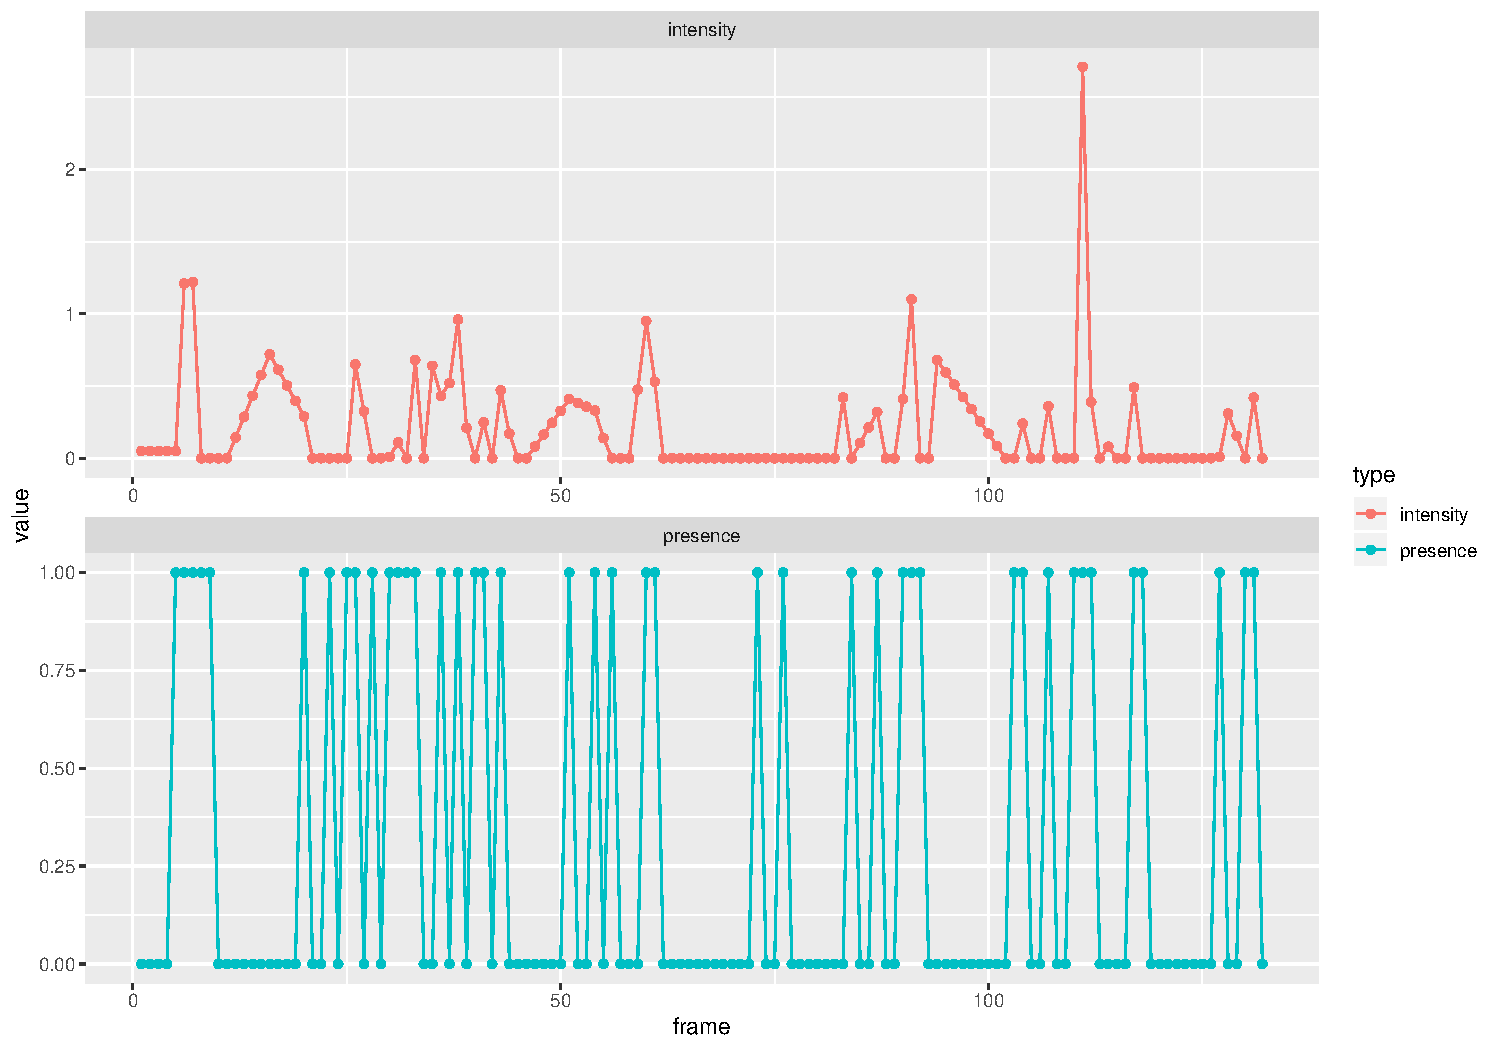
\includegraphics[width=1\linewidth]{figures/ts-plot-1} 

}

\caption{The plot shows the intensity and presence score of action unit 01 for Justices Edelman in case McKell in a time series manner. }\label{fig:ts-plot}
\end{figure}

\hypertarget{missing-value-imputation}{%
\section{Missing value imputation}\label{missing-value-imputation}}

The missingness in the dataset could be due to the fact that a judge is reading the materials on the desk so the face is not captured for a particular frame or simply because some faces are not detectable for the given resolution of the video stream. Simply drop the missing observation will cause the time interval to be irregular and thus imputation is needed.

Intensity is a continuous variable that measures how strong the action unit is presented. It is zero when the action unit is not present, 1(present at minimum intensity) to 5(present at maximum intensity). Linear interpolation function (\texttt{na.interp()}) from \texttt{forecast} package is used to impute Intensity. The missing value of presence is then imputed based on if the intensity score of the missing observations are greater than one.

\hypertarget{source-code}{%
\section{Source Code}\label{source-code}}

The whole data processing procedure is done as a major part of the project and one of the difficulties of this project is actually to source reliable facial data of the judges, so that the subsequent modelling can then be conducted meaningfully. The whole workflow has been scripted and labelled accordingly from \texttt{data\_01...} to \texttt{data\_07...} on my github repository. If re-processing is needed, or more videos need to be added, it is straightforward for others to do.

\hypertarget{methodology}{%
\chapter{Methodology}\label{methodology}}

\hypertarget{notation}{%
\section{Notation}\label{notation}}

Let \(\mathbf{X}\) be a matrix of predictors, and \(\mathbf{Y}\) variable in our case is bivariate matrix of response variables, including a binary indicator of presence/absence and a numeric value measuring intensity, of facial action unit, where

\begin{itemize}
\tightlist
\item
  \(X_1\) indicates \texttt{judge} with six categories \(i = 1,2, \cdots, 6\)
\item
  \(X_2\) indicates \texttt{video} for each of the seven cases, \(j = 1,2, \cdots, 7\)
\item
  \(X_3\) indicates action unit containing 18 possible facial expression.\\
\item
  \(X_4\) indicates \texttt{speaker}, either the appellant or respondent, \(l=1,2\)
\item
  \(X_5\) indicates \texttt{frame} corresponding to time, \(t = 1,2, \cdots, T_j\)
\end{itemize}

Note that \(t\) could be considered a time variable, but because images are taken at 1 minute intervals, temporal dependence is unlikely to exist. Rather this should be considered an independent observation.

A full, main effects model for the data might be expressed as:

\[Y_{ijklt} = \mu + \alpha_i + \beta_j + \gamma_k + \delta_l + \varepsilon_{ijklt}\]

\noindent Also, let \(P_{jitkl}\) represent the response variable presence, and \(I_{jitkl}\) represent the response variable intensity. This notation will be helpful for defining the plots and models explained in this section.

\hypertarget{modelling-presence}{%
\section{Modelling Presence}\label{modelling-presence}}

\hypertarget{model-structure}{%
\subsection{Model structure}\label{model-structure}}

The presence score is a binary variable that is one when a particular action unit is observed and zero if not. This suggests using a logistic model and we implement this using the \texttt{glm()} function from base R. The link function of a matter of choice in the \texttt{glm()} function and the logit link is chosen because it is the canonical link of the binomial family. An alternative link could be a probit link but theoratically, these two links give very similar result in terms of prediction \textcite{faraway2016extending}. The structure of the model is written as in Equation \ref{eq:logit-structure} with the first equation linking the mean of the presence to the linear prediction and the second equation specifying the linkage between \(\eta\) to the predictors. The next section will specify three different function form of the linear predictor by introducing different variables and interactions.

\begin{align}\label{eq:logit-structure}
\mu &= \frac{e^{\eta}}{1 + e^{\eta}} \\
\eta &= f(\alpha_i\text{,}\beta_j\text{,}\gamma_k\text{,}\delta_l)
\end{align}

\hypertarget{model-1-action-unit}{%
\subsection{Model 1: Action unit}\label{model-1-action-unit}}

The first linear function is written in Equation \ref{eq:judge_au}. It includes the main effect of judge and action unit and also their interaction. Interaction terms are included to capture the judge-wise differences for different action units and it is necessary because we suspect different judges could have different average presence scores for different action units.

\begin{align}\label{eq:judge_au}
\eta_{ik} &= \mu + \alpha_i + \gamma_k + (\alpha\gamma)_{ik}
\end{align}

\hypertarget{model-2-video}{%
\subsection{Model 2: Video}\label{model-2-video}}

Build upon the first model, the second model adds the video related main effect and interactions, as shown in Equation \ref{eq:judge_video}. The interactions allow both judge and action unit variables to differ in different videos, which is useful to answer the research questions \emph{whether the judges are behaving same or different across videos}.

\begin{align}\label{eq:judge_video}
\eta_{ijk} &= \mu + \alpha_i + \beta_j +\gamma_k + (\alpha\beta)_{ij} + (\alpha\gamma)_{ik} + (\beta\gamma)_{jk}
\end{align}

\noindent 

\hypertarget{model-3-speaker}{%
\subsection{Model 3: Speaker}\label{model-3-speaker}}

Build upon the second model, the third model is aimed to capture the speaker-wise effect by including the judge and speaker interaction as in Equation \ref{eq:judge_speaker}. This model would be helpful to answer the question \emph{do the expressions of the judges change when different parties are speaking}. The reason for not including more interaction between speaker and video or action unit is because this could cause the model to run out of degree of freedom given the number of observations we have.

\begin{align}\label{eq:judge_speaker}
\eta_{ijkl} &= \mu + \alpha_i + \beta_j +\gamma_k + \delta_l + (\alpha\beta)_{ij} + (\alpha\gamma)_{ik} + (\beta\gamma)_{jk} + (\alpha\delta)_{il}
\end{align}

\hypertarget{analysis-of-variance-anova}{%
\subsection{Analysis of variance (ANOVA)}\label{analysis-of-variance-anova}}

The analysis of variance (ANOVA) \autocites{faraway2016extending}{gelman2006data} is a statistical method that can be used to compare different models. Different packages in R conduct ANOVA test: \texttt{anova()} and \texttt{drop()} from base R, \texttt{Anova()} from \texttt{car} package and \texttt{aov()} from \texttt{stats} package. We use the base R \texttt{anova()} function to compare the three models via chi-square tests.

\newpage

\hypertarget{modelling-intensity}{%
\section{Modelling Intensity}\label{modelling-intensity}}

The intensity score is a continuous variable starts from zero when the action unit is not present to 5, where an action unit is presented at maximum intensity. A histogram of the intensity is plotted in Figure \ref{fig:intensity} and the distribution has a high proportion of zeros with highly skewed continuous value. This type of data is the so-called semi-continuous data \autocites{Neelon2019}{twopart2010}. The semi-continuous data can be modelled in the econometrics literature by the two part model\autocites{cragg1971some}{manning1981two}. In the two part model, the data is viewed to be generated via a sequential modelling technique, which is a mixed distribution of

\begin{itemize}
\tightlist
\item
  a logistic model of if Y = 0 or not, and
\item
  a specific model for the conditional distribution of \(y \mid y > 0\).
\end{itemize}

\begin{figure}

{\centering 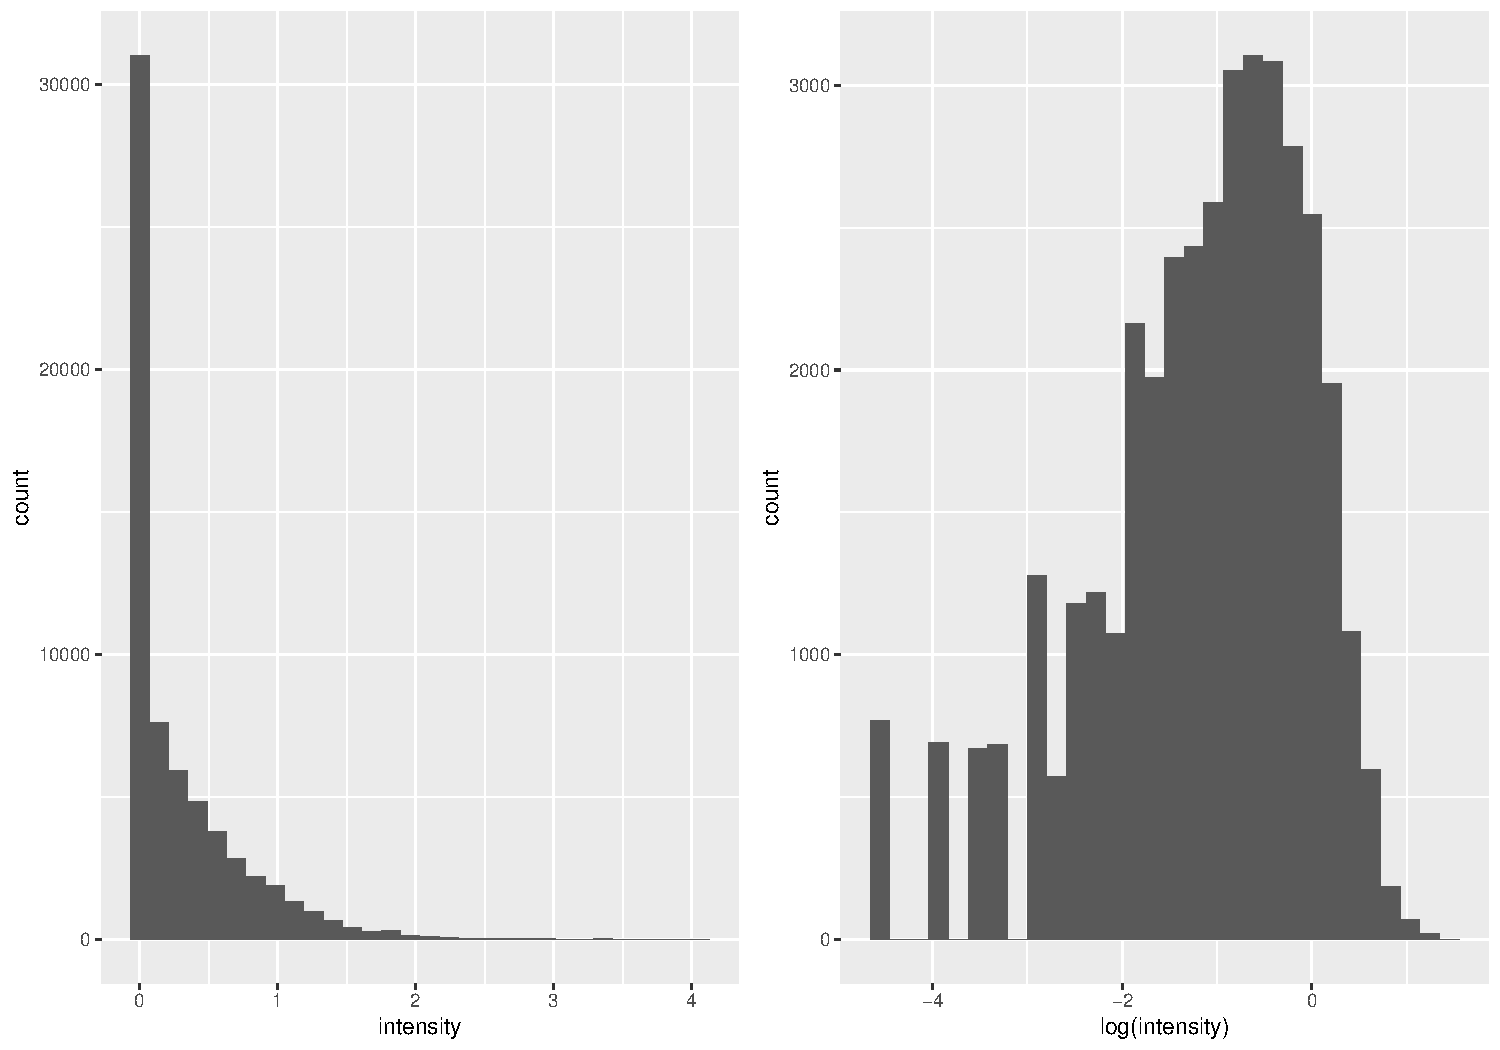
\includegraphics[width=1\linewidth]{figures/intensity-1} 

}

\caption{From the histogram of the intensity score, the data is highly skewed with an excessive amount of zeros. The two part model is about to accommodate the excessive zeros via the logistic model and gamma regression is about to capture the skewness in the data.}\label{fig:intensity}
\end{figure}

The choice of model between two part model and sample selection model is always discussed in the literature. Monte-Carlo simulation studies by different researchers \autocites{leung1996choice}{duan1984choosing}{manning1987monte} show different results on whether these different classes of model are answering the same or distinct inferential questions. The reason for us to choose two part model rather than sample selection model is because the problem of not being able to observe \(Y\) for those observations with selection variable \(z = 0\) doesn't exist in our data. In another word, if an action unit is not present for an observation, it doesn't make sense to talk about ``intensity score if the action unit is present''. Tobit model is not appropriate because the data can't be viewed as normally distributed with negative value censored as zero (meaningless to say negative intensity value). Zero inflated model is not used because it considers two source of zeros in the data while there is no zeros being generated from the second model (only one source of zeros).

The two part model has a general structure as in Equation \ref{eq:two-part-general}.

\begin{align}\label{eq:two-part-general}
\mu^1 &= \frac{e^{\eta}}{1 + e^{\eta}} \\
\eta &= f(\alpha_i, \beta_j, \gamma_k, \delta_l) \\
\mu^2 &= \log(I) \\
E(I \mid I > 0) &= f(\alpha_i, \beta_j, \gamma_k, \delta_l)
\end{align}

\noindent The first two equations capture the logistic link and its linear predictor. The next two specify the functional form of the conditonal distribution. The functional form of the conditional distribution need to be able to capture the highly skewed nature of the non-zero observations. A convention approach is to assume the conditional distribution is a lognormal distribution \autocites{manning1981two}{diehr1999methods}. More recent literature proposes the use of gamma or generalised gamma regression model for the conditional distribution \autocite{twopart2010}. Gamma regression is used to because it could also capture the right skewness and it is easier to implement via the \texttt{glm()} function. The log link function is used because the canonical inverse link for gamma distribution will cause some estimated marginal mean to be extremely high and thus meaningless for intensity score.

The linear predictor of the conditional intensity that includes video and relevant interactions is written in Equation \ref{eq:two-part1}.

\begin{align}\label{eq:two-part1}
E(I_{ijk} \mid I_{ijk} > 0) &= \mu + \alpha_i + \beta_j +\gamma_k + (\alpha\beta)_{ij} + (\alpha\gamma)_{ik} + (\beta\gamma)_{jk}
\end{align}

The model that captures additional speaker variable is written in Equation \ref{eq:two-part2}.

\begin{align}\label{eq:two-part2}
E(I_{ijkl} \mid I_{ijkl} > 0) &= \mu + \alpha_i + \beta_j +\gamma_k + \delta_l + (\alpha\beta)_{ij} + (\alpha\gamma)_{ik} + (\beta\gamma)_{jk} + (\alpha\delta)_{il}
\end{align}

\newpage

\hypertarget{post-model-analysis}{%
\section{Post-Model Analysis}\label{post-model-analysis}}

The estimates of variables from the model summary are not particularly useful in our case. This is because firstly, the estimates of the coefficient are not interpretable in the logistic regression. Secondly, we are interested in whether the mean for each treatment is same or different. To assess which level of the factor is different requires post-model analysis.

\hypertarget{estimated-marginal-mean-emm}{%
\subsection{Estimated Marginal Mean (EMM)}\label{estimated-marginal-mean-emm}}

The estimated marginal mean \autocite{gelman2006data} is the fitted value from a model over the treatmetn effects. In our data, the treatment effects include judge, video and action unit. The estimated marginal mean is computed using \texttt{emmean()} from the \texttt{emmenas} package. The probability from estimated marginal mean have a nice interpretation as the estimated probability of presence score for a particular combination of action unit, judge and video. This output allows us to compare how the estimated presence probabilities of each judge, video and action unit combination are different or similar from each other.

\hypertarget{confidence-interval-adjustment}{%
\subsection{Confidence Interval Adjustment}\label{confidence-interval-adjustment}}

Testing significance based on p-value has been long criticised for its interpretation. Researchers can erroneously conclude significance because of p-value being less than 0.05 without discussing the false positive/negative proportion. On the other hand, confidence interval provides a confidence range for the estimates to highlight the uncertainty around estimation. Thus confidence interval is used to compare whether the estimated mean for a particular judge-AU group is same or different across videos based on if the intervals overlap with each other.

The confidence intervals computed from the \texttt{emmean()} function need to be adjusted for simultaneous inference. A 5\% significance level indicates if we conduct 100 tests simultaneously, about 5 tests will show significance out of randomness. This is a problem we need to pay attention to when comparing the estimated presence probability or we may wrongly conclude judges has a different facial expression than others but they are actually not.

When multiple estimated mean are compared at the same time, the confidence level (or \(\alpha\) in p-value) need to be adjusted to control the family-wise error rate to be less than \(\alpha\). Bonferroni adjustment makes the adjustment to reject a hypothesis test at \(\alpha/N\) level so that the type I error of whole family of the simultaneous tests (Family-wise Error Rate (FWER)) is control be less than \(\alpha\). To do this, \texttt{confint()} function from base R is used with additional argument \texttt{adjust\ =\ "bonferroni"}.

\hypertarget{results}{%
\chapter{Results}\label{results}}

\hypertarget{exploratory-data-analysis}{%
\section{Exploratory Data Analysis}\label{exploratory-data-analysis}}

\hypertarget{action-unit-presence}{%
\subsection{Action unit: Presence}\label{action-unit-presence}}

\hypertarget{mean-presence-score-and-most-common-action-units}{%
\subsubsection{Mean presence score and most common action units}\label{mean-presence-score-and-most-common-action-units}}

The average presence (\(P_{ik}\)) of each action unit is first computed for each judge as \[P_{ik} = \frac{\sum_{jt}X_{ijtk}}{\sum_{j = 1}^JT_j}\] This is plotted in Figure \ref{fig:mean_presence} to give an overview of the presence score of all the action units across all the judges. The order of action unit on the y axis is ranked by the average presence of all the judges. The five most frequent action units are highlighted in blue for each judge and summarised in Table \ref{tab:most_common}

\begin{figure}

{\centering 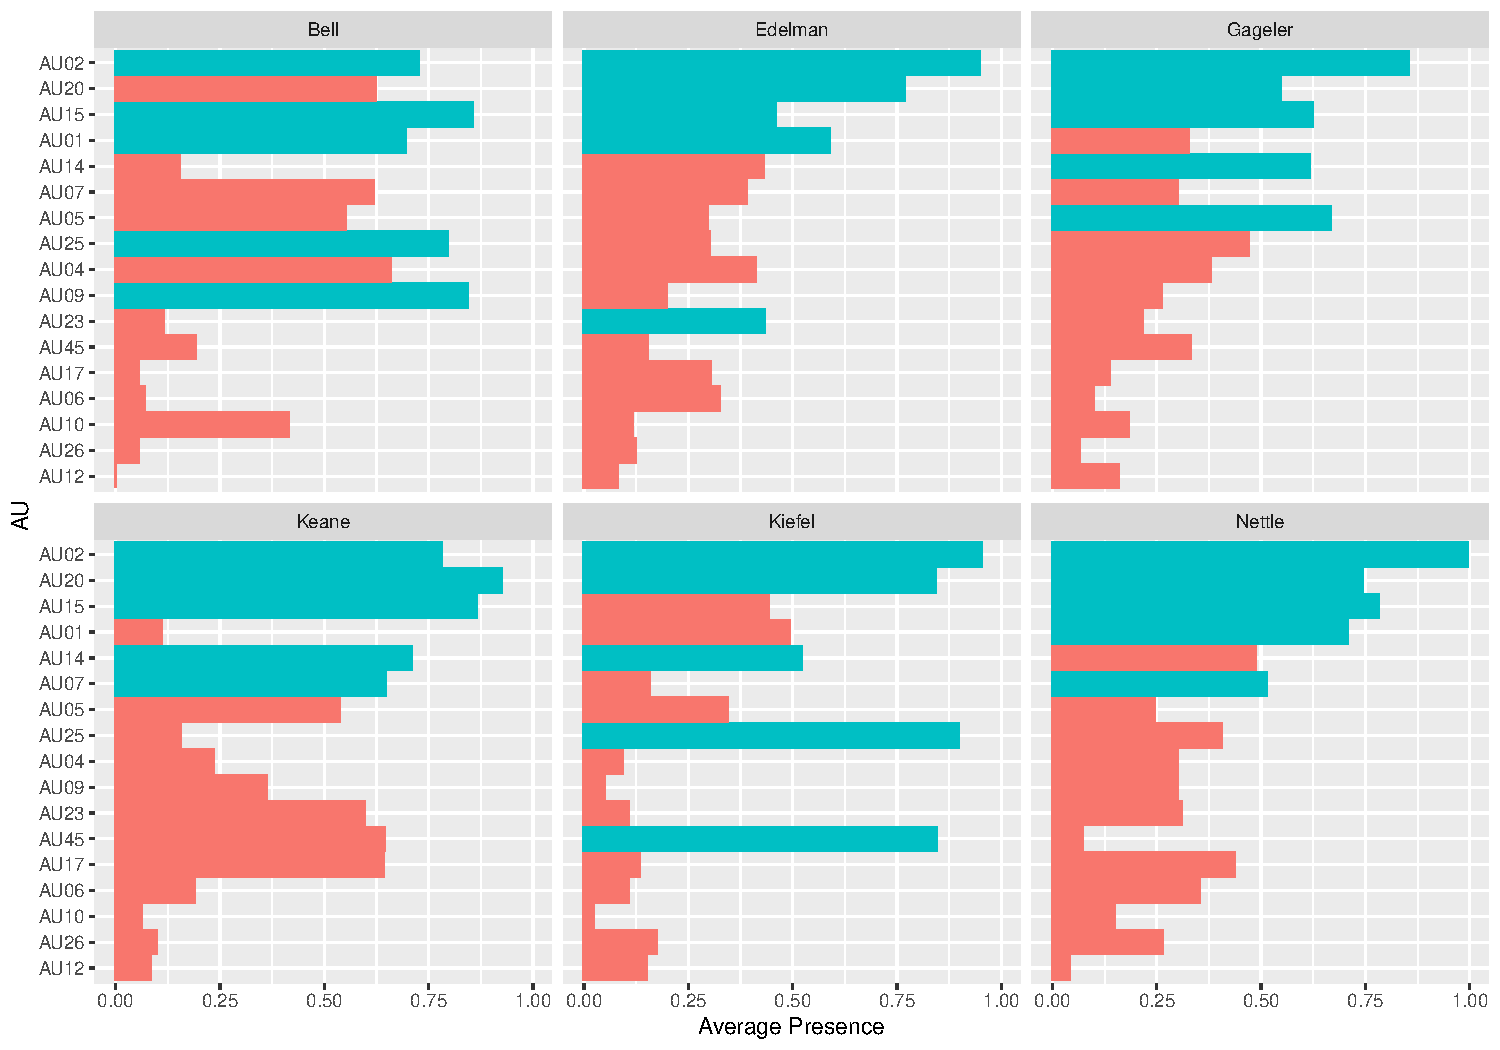
\includegraphics[width=1\linewidth]{figures/most-common-1} 

}

\caption{The average presence score of each action unit for each judge, aggregating on video and time. \label{fig:mean_presence}}\label{fig:most-common}
\end{figure}

\begin{table}[ht]
\begin{center}
\caption{\label{tab:most_common}The five most commonly presented action units for each judge.}
\begin{tabular}{rllllll}
\toprule
index & Bell & Edelman & Gageler & Keane & Kiefel & Nettle \\
\midrule
1 & AU15 & AU02 & AU02 & AU20 & AU02 & AU02 \\
2 & AU09 & AU20 & AU05 & AU15 & AU25 & AU15 \\
3 & AU25 & AU01 & AU15 & AU02 & AU45 & AU20 \\
4 & AU02 & AU15 & AU14 & AU14 & AU20 & AU01 \\
5 & AU01 & AU23 & AU20 & AU07 & AU14 & AU07 \\
\bottomrule
\end{tabular}
\end{center}
\end{table}

It can be seen that some of the action units are common across almost all the judges, these includes AU02 (outer eyebrow raise), AU20 (lip stretcher), AU15 (Lip Corner Depressor) and AU14 (Dimpler).

According to \textcite{ekman2002facial}, AU02 makes a contribution to surprise, which may be a positive attitude showing that judges are interested in a particular moment. AU14 indicates boredom and AU15 shows confusion. Based on the most common five action units, the emotions judges displayed in the courtroom can be summarised into three categories, described in Table \ref{tab:three_category}, along with the featured action units.

\hypertarget{presence-by-videos}{%
\subsubsection{Presence by videos}\label{presence-by-videos}}

We are also interested in the main presence score of the judges by video (\(P_{ijk}\)). This is computed as \[P_{ijk} = \frac{\sum_{t}X_{ijtk}}{T_j}\] for the four most common action units: AU02, AU14, AU15, AU20 and plotted in Figure \ref{fig:common_video}. From this plot, we can observe that some Justices have larger fluctuation of their expression of action units while others are more consistent throughout different videos. For example, Justice Gageler, coloured as green, has a much higher proportion of expression in case OKS, especially in action unit 14, 15 and 20. Justices Bell, who is coloured red has the highest proportion of expression in case OKS while lowest in case Parkes for action unit 14 and 20.

\begin{figure}

{\centering 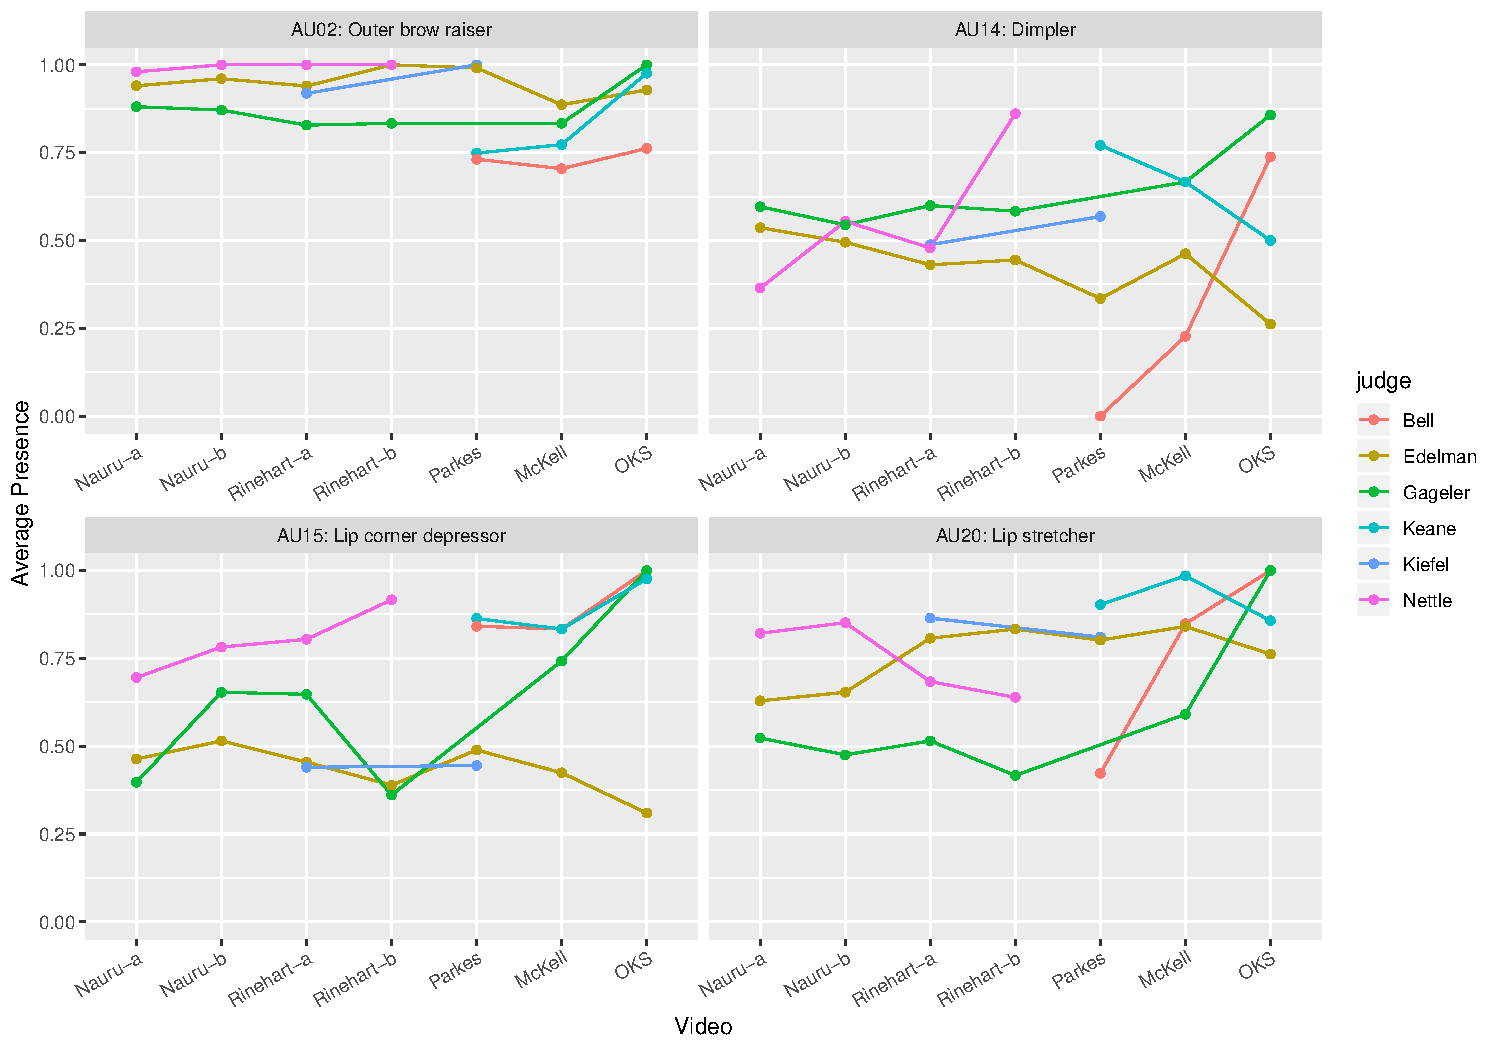
\includegraphics[width=1\linewidth]{figures/au-video-1} 

}

\caption{Average presence of the four most common action units for each judge by video\label{fig:common_video}}\label{fig:au-video}
\end{figure}

\hypertarget{action-unit-intensity}{%
\subsection{Action unit: Intensity}\label{action-unit-intensity}}

\hypertarget{general-intensity-plot}{%
\subsubsection{General Intensity plot}\label{general-intensity-plot}}

The boxplot of the intensity for all the judges across all the videos is presented in Figure \ref{fig:intensity}. Each bar-and-whisker represents the intensity (\(I_{ijtk}\)) of all the action units aggregated on time for a particular judge \(i\) in a specific case \(j\). For example, the first bar-and-whisker in case Nauru\_a is created using all the 17 action units of Edelman through out the elapsed time in Nauru\_a case. The square root transformation is applied so that the mean of the intensity can be easier to be visualised. From the plot, we can see that most of the action units have low intensity score and this is expected because usually judges are expected not to express to much of their expressions in the court room. We can find that Justices Nettle, colored pink seems to have higher average in all the four cases he appeared.

\begin{figure}

{\centering 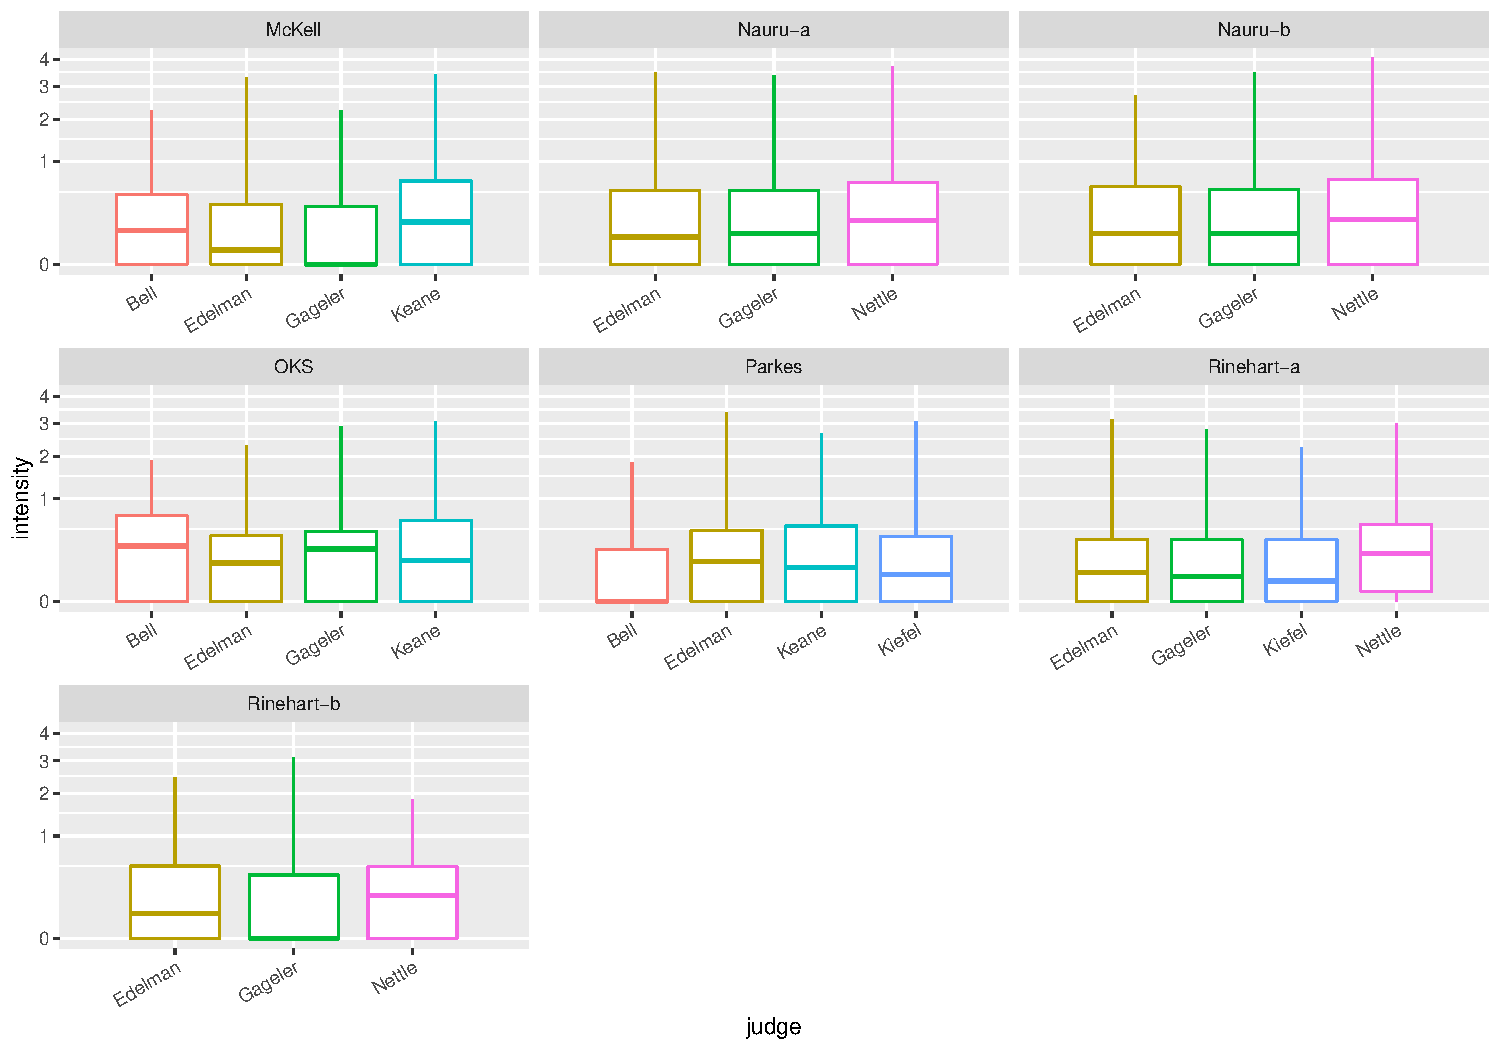
\includegraphics[width=1\linewidth]{figures/intensity-boxplot-1} 

}

\caption{General intensity score by judge and video\label{fig:intensity}}\label{fig:intensity-boxplot}
\end{figure}

\hypertarget{mean-intensity}{%
\subsubsection{Mean intensity}\label{mean-intensity}}

Mean intensity score (\(I_{ik}\)) of each action unit for each of the judge is computed as \[I_{ik} = \frac{\sum_{jt}X_{ijtk}}{\sum_{j = 1}^JT_j}\] and plotted in Figure \ref{fig:mean_intensity}. The five most intense action units for each judge are presented in Table \ref{tab:most_intense}. We can find that the most common high intense action units includes AU20 (Lip Stretcher), AU07 (Lid Tightener) and AU04 (Brow Lower).

\begin{figure}

{\centering 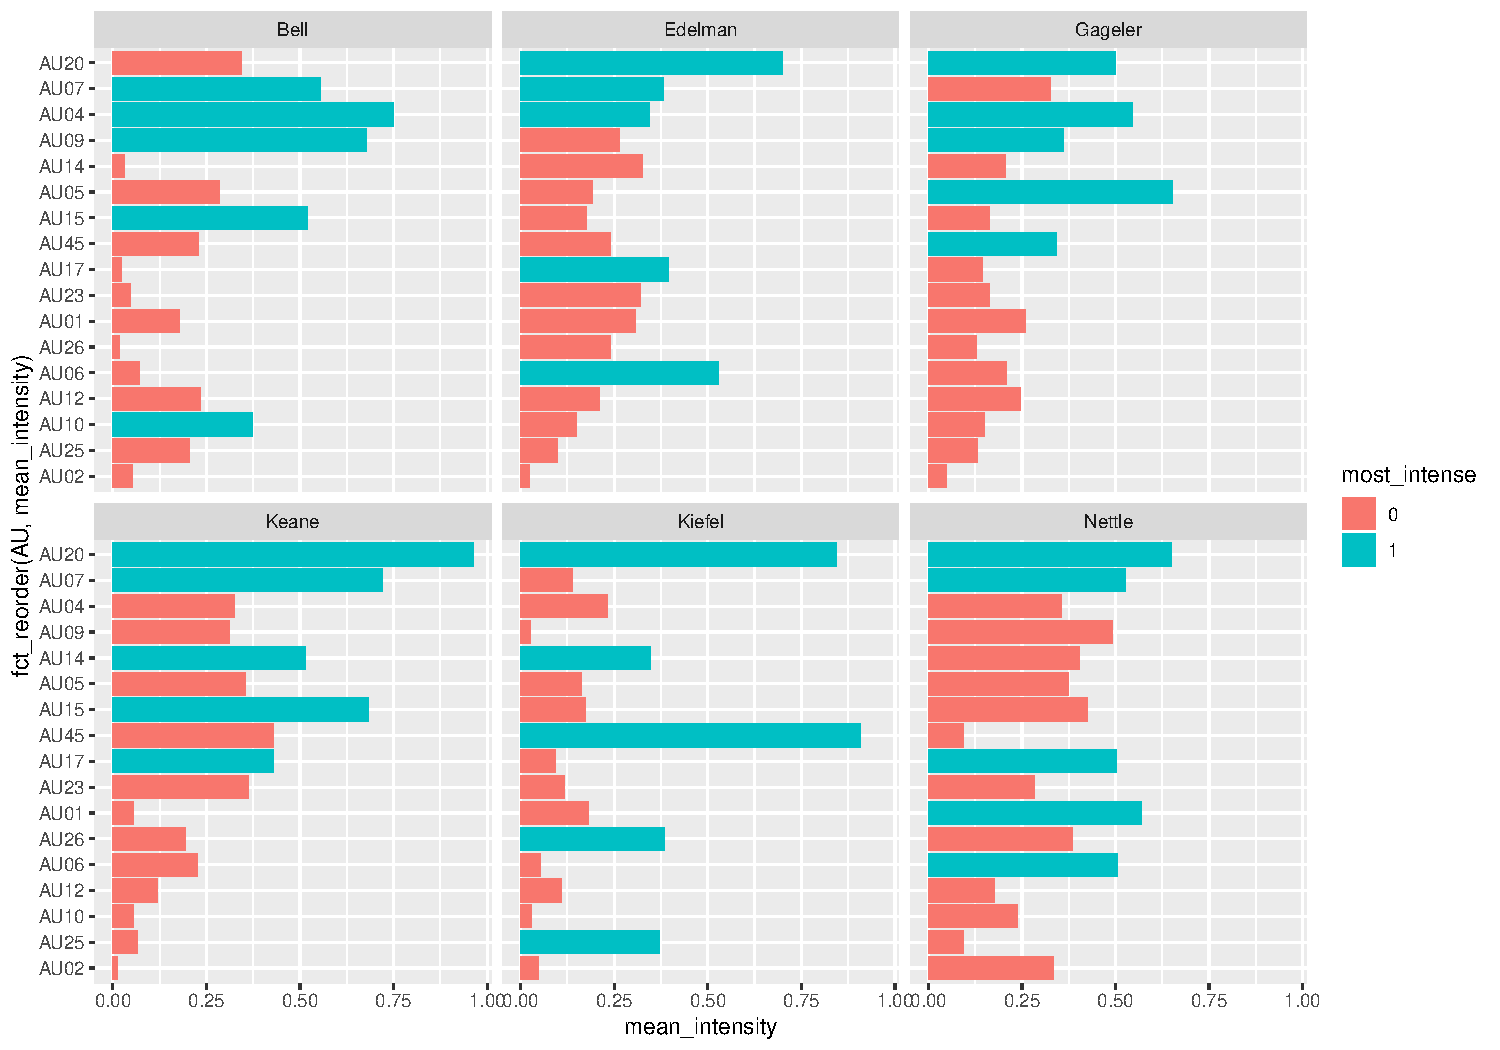
\includegraphics[width=1\linewidth]{figures/mean-intensity-1} 

}

\caption{Mean intensity score for each judge and action unit aggregating on videos.\label{fig:mean_intensity}}\label{fig:mean-intensity}
\end{figure}

\begin{table}[ht]
\begin{center}
\caption{\label{tab:most_intense}The five most intense action unit for each judge.}
\begin{tabular}{rllllll}
\toprule
index & Bell & Edelman & Gageler & Keane & Kiefel & Nettle \\
\midrule
1 & AU04 & AU20 & AU05 & AU20 & AU45 & AU20 \\
2 & AU09 & AU06 & AU04 & AU07 & AU20 & AU01 \\
3 & AU07 & AU17 & AU20 & AU15 & AU26 & AU07 \\
4 & AU15 & AU07 & AU09 & AU14 & AU25 & AU06 \\
5 & AU10 & AU04 & AU45 & AU17 & AU14 & AU17 \\
\bottomrule
\end{tabular}
\end{center}
\end{table}

\hypertarget{high-intensity-points}{%
\subsubsection{High intensity points}\label{high-intensity-points}}

I also plotted the points with intensity greater than two against time for all the justices in Figure \ref{fig:high-intensity-points}. It tells us that Edelman, Gageler and Nettle are the judges have stronger emotion that can be detected since they have more points with intensity greater than 2. Different judges also have different time where they display stronger emotions. For example, Justice Edelman are more likely to have stronger emotion throughout the time while Justices Nettle is more likely to have intense facial expressions at the beginning and ending of the hearing.

\begin{figure}

{\centering 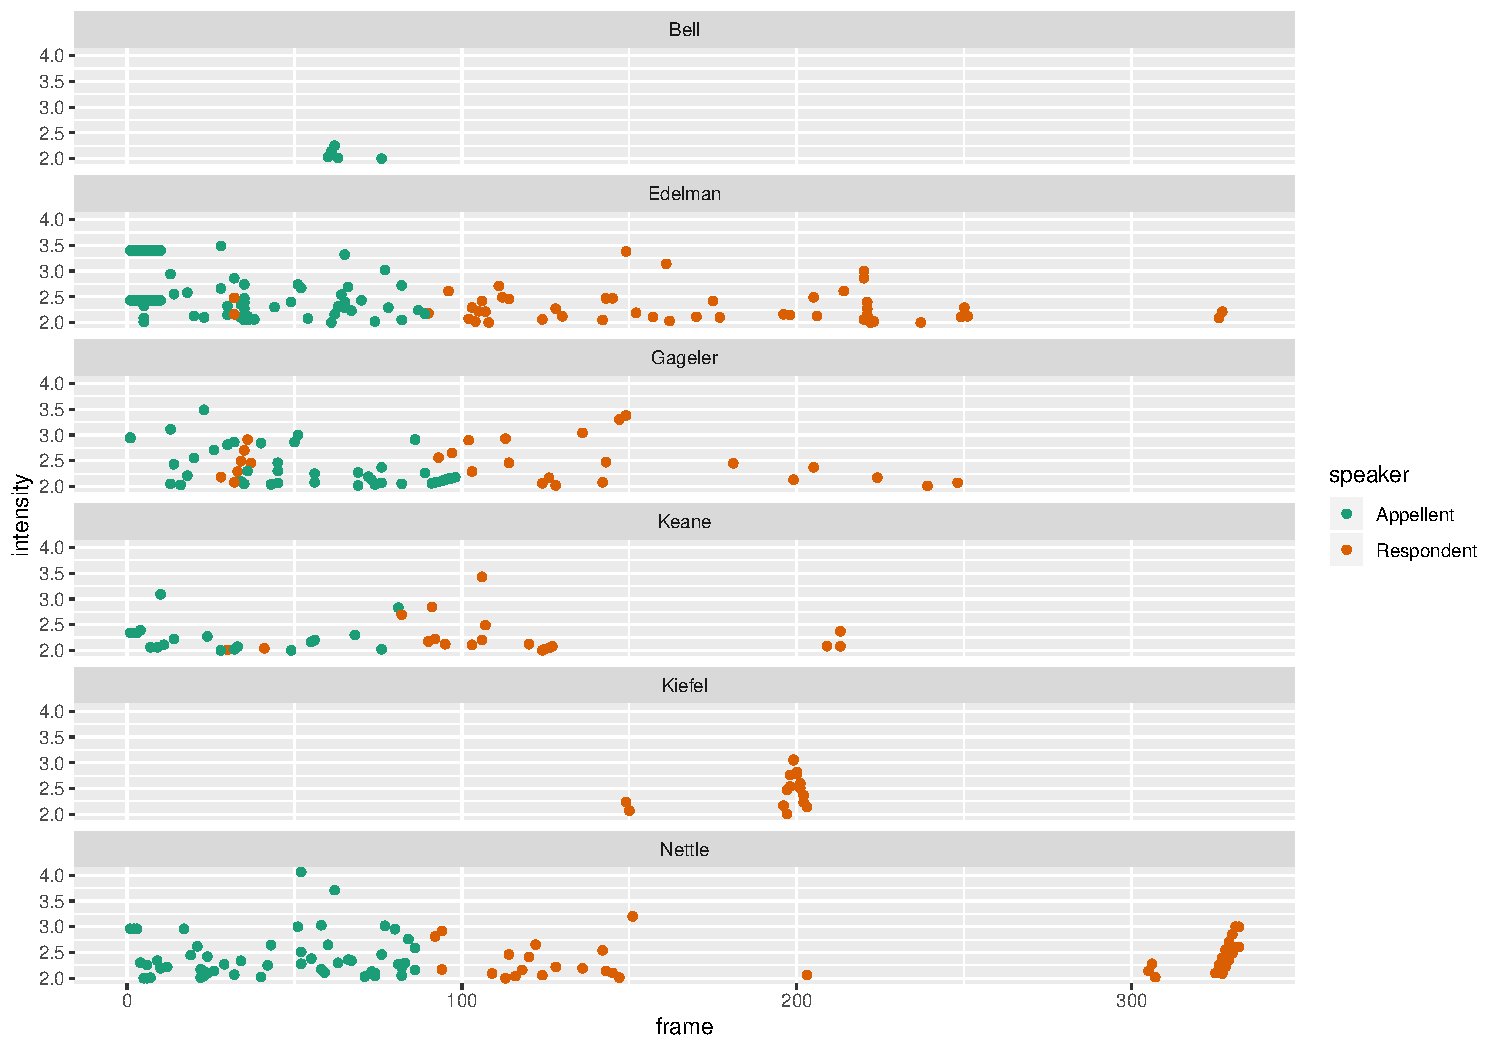
\includegraphics[width=1\linewidth]{figures/high-intensity-points-1} 

}

\caption{this is the plot}\label{fig:high-intensity-points}
\end{figure}

\hypertarget{summary}{%
\subsection{Summary}\label{summary}}

The findings from the exploratory data analysis are summarised below

\begin{itemize}
\item
  The most common action unit from the Justices are AU02 (outer eyebrow raise), AU20 (lip stretcher), AU15 (Lip Corner Depressor) and AU14 (Dimpler).
\item
  Some Justices show relatively consistent facial expression through different videos while others, for example Justices Gageler and Bell have larger fluctuation on their facial expressions in different cases.
\item
  The overall intensity of the action units are low while Justices Nettle seems to have a relatively higher intensity than other Justices.
\item
  Edelman, Gageler and Nettle are the Justices with more intense facial expressions in the courtroom and Justices Nettle is the only Justice that tends to have stronger expression towards the end of the hearing.
\end{itemize}

\newpage

\hypertarget{choice-of-action-unit-to-include}{%
\section{Choice of action unit to include}\label{choice-of-action-unit-to-include}}

The number of action unit to include in the model is a matter of choice. The discussion of this choice is to ensure our model is parsimonious, that is, a model has the smallest number of variables but with greatest explanatory power. Random effect is a way to deal with large number of factor levels of a variable, but in our context, we are only interested in the action units with a certain mean presence (and intensity) for most of the judges.

The mean presence and intensity score for each action unit is computed and the action units to include in the model are the ones that appear in the top 10 action unit for both mean presence and intensity rank. This ensures that these action units have both relativcely high intensity and presence score. A list of included action units along with their meaning and related emotions are presented in Table \ref{tab:au-included}

\begin{table}[ht]
\begin{center}
\caption{\label{tab:au-included} These are the selected action units that will be included in the modelling for intensity and presence.}
\begin{tabular}{lll}
\toprule
AU-number & meaning & emotion \\
\midrule
AU01 & Inner brow raiser & sadness, surprise and fear \\
AU04 & Brow lowerer & sadness, fear, anger and confusion \\
AU05 & Upper lid raiser & surprise, fear, anger adn interested \\
AU07 & Lid tightener & fear, anger and confusion \\
AU14 & Dimpler & contempt or boredom if appears unilateraly \\
AU15 & Lip corner depressor & sadness, disgust and confusion \\
AU20 & Lip stretcher & fear \\
AU45 & Blink & NA \\
\bottomrule
\end{tabular}
\end{center}
\end{table}

\newpage

\hypertarget{modelling-result-for-presence-intensity}{%
\section{Modelling result for presence \& intensity}\label{modelling-result-for-presence-intensity}}

\hypertarget{model-fitting-and-anova}{%
\subsection{Model fitting and ANOVA}\label{model-fitting-and-anova}}

The three models in Equation \ref{eq:judge_au}, \ref{eq:judge_video} and \ref{eq:judge_speaker} has been fitted and ANOVA test is performed to choose the best model. In Table \ref{tab:anova-1}, the deviance of model 1 and 2 are compared and the p-value rejects the null hypothesis that model 1 and model 2 are the same. The comparison of model 2 and model 3 is presented in Table \ref{tab:anova-2}. We take a conservative approach and not rejecting the null hypothesis that model 3 is too much different from model 2. Thus, model 2 is chosen as our final model for modelling presence.

\begin{table}[ht]
\begin{center}
\caption{\label{tab:anova-1}this is the caption}
\begin{tabular}{lllll}
\toprule
Resid. Df & Resid. Dev & Df & Deviance & Pr(>Chi) \\
\midrule
30320 & 35850 & NA &    NA &        NA \\
30259 & 35256 & 61 & 594.4 & 1.793e-88 \\
\bottomrule
\end{tabular}
\end{center}
\end{table}

\begin{table}[ht]
\begin{center}
\caption{\label{tab:anova-2}this is the caption}
\begin{tabular}{lllll}
\toprule
Resid. Df & Resid. Dev & Df & Deviance & Pr(>Chi) \\
\midrule
30259 & 35256 & NA &    NA &      NA \\
30253 & 35242 &  6 & 14.21 & 0.02742 \\
\bottomrule
\end{tabular}
\end{center}
\end{table}

\hypertarget{residual-diagnostics-and-post-model-analysis}{%
\subsection{Residual Diagnostics and post-model analysis}\label{residual-diagnostics-and-post-model-analysis}}

Residual analysis is performed on model 2 to illustrate the fitness of the model. In Figure \ref{fig:resid}, the left panel shows the residual for each judge in a boxplot and one can observe that the residuals are around zero for most of the Justices. On the right panel, the residuals are plotted as dots and there is no pattern shown on the plot. This indicates model 2 has a good fit.

\begin{figure}

{\centering 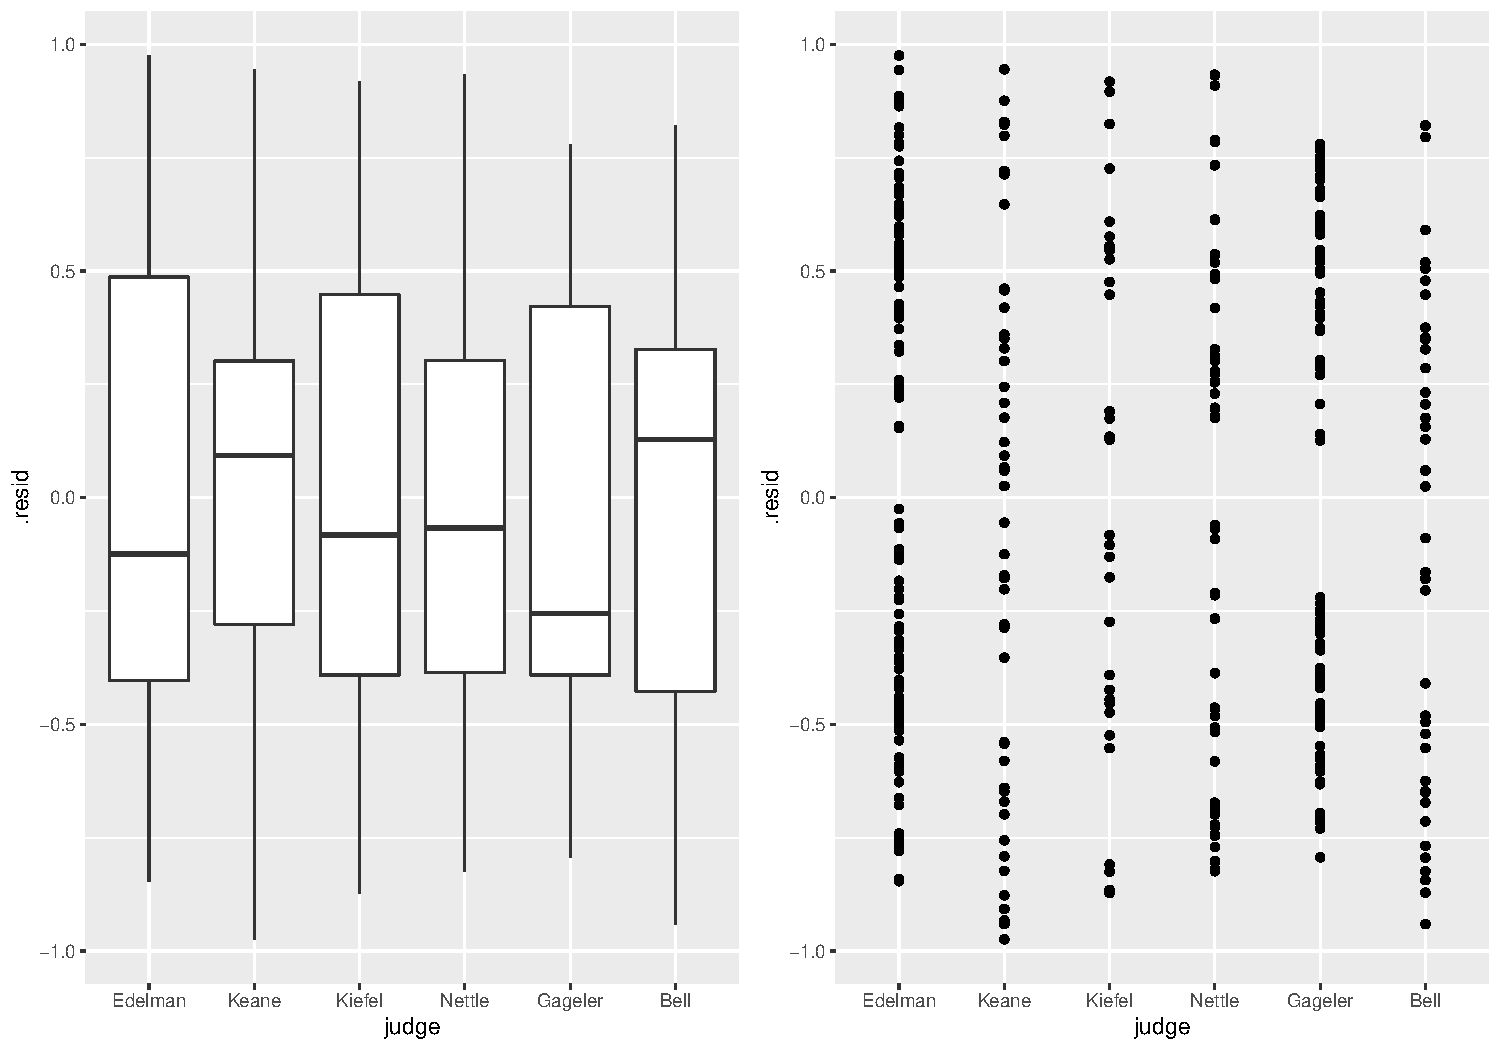
\includegraphics[width=1\linewidth]{figures/resid-1} 

}

\caption{The residual plot for model 2. }\label{fig:resid}
\end{figure}

The estimated marginal mean is computed in Table \ref{tab:result-2} in the Appendix The \texttt{prob} column can be interpreted as after averaging over all the videos and speaking parties, the estimated mean probability for judge Edelman in action unit AU02 is 0.95, with a 95\% confidence interval of {[}0.92, 0.97{]}. Notice that confidence intervals for a generalised linear model is asymmetric around the estimates because the linear symmetric interval of the mean need to be transferred via the inverse of link function to get the confidence interval for the response. The 95\% confidence interval after bonferroni adjustment is plotted in Figure \ref{fig:model2-plot}.

\begin{figure}

{\centering 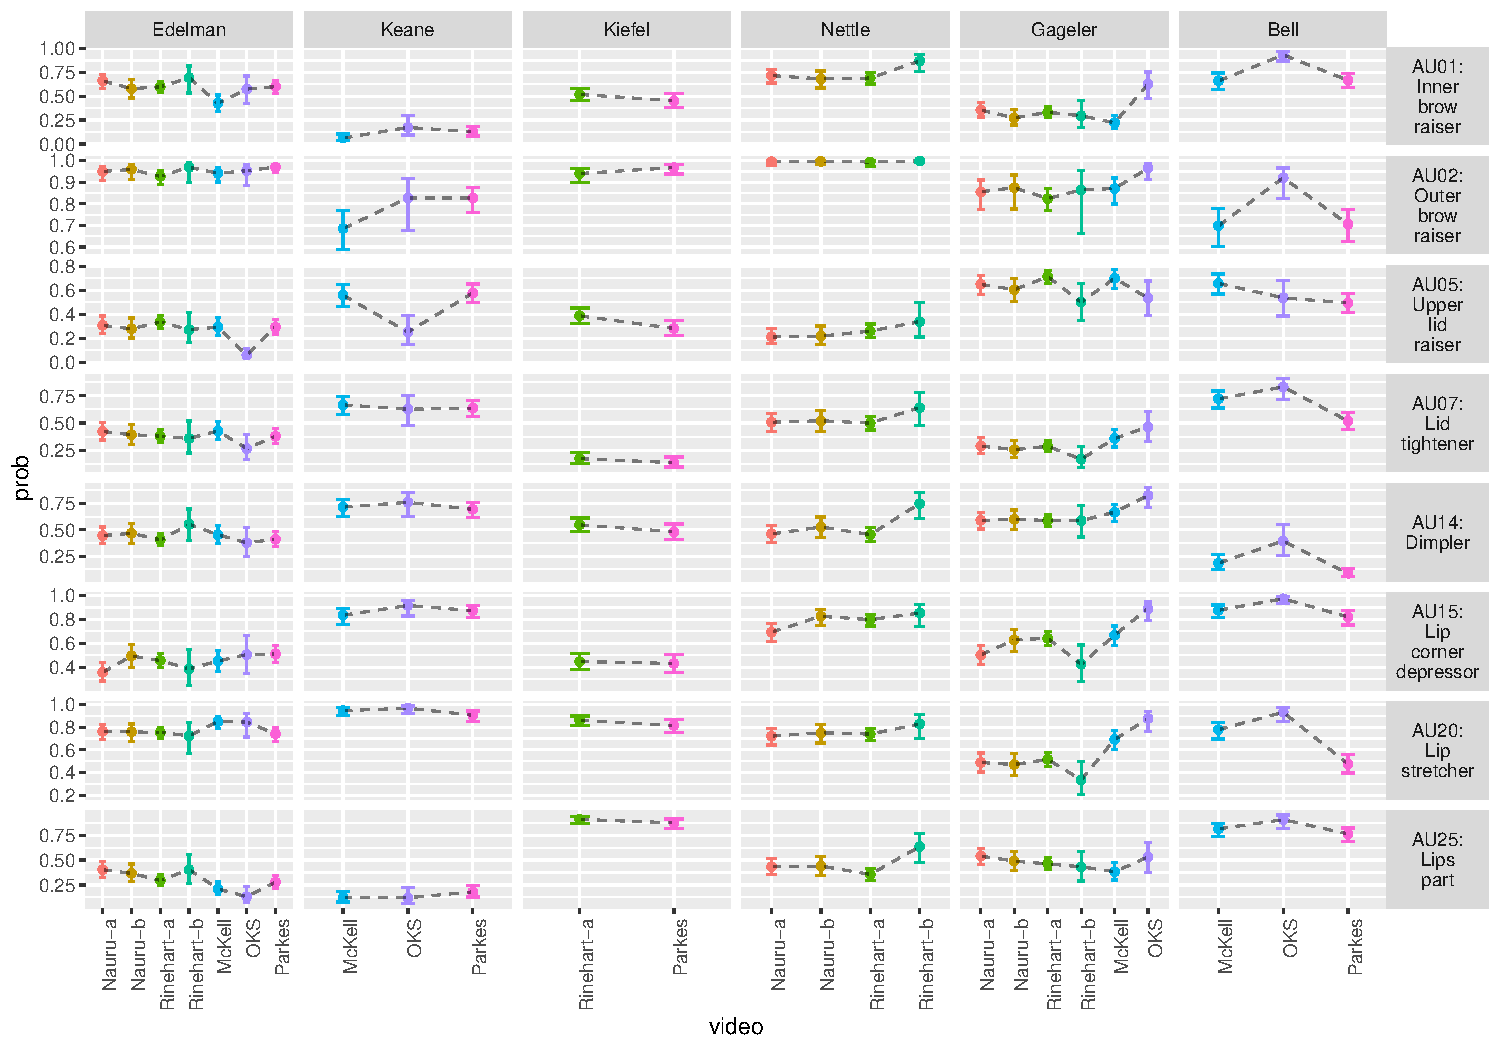
\includegraphics[width=1\linewidth]{figures/model2-plot-1} 

}

\caption{The confidence interval for estimated mearginal mean in model 2}\label{fig:model2-plot}
\end{figure}

The two part model in equation \ref{eq:two-part1} is estimated for the intensity data. Estimated marginal mean and confidence interval adjustment procedure are performed as modelling presence data. The 95\% confidence interval plot is presented in Figure \ref{fig:intensity-video}.

\begin{figure}

{\centering 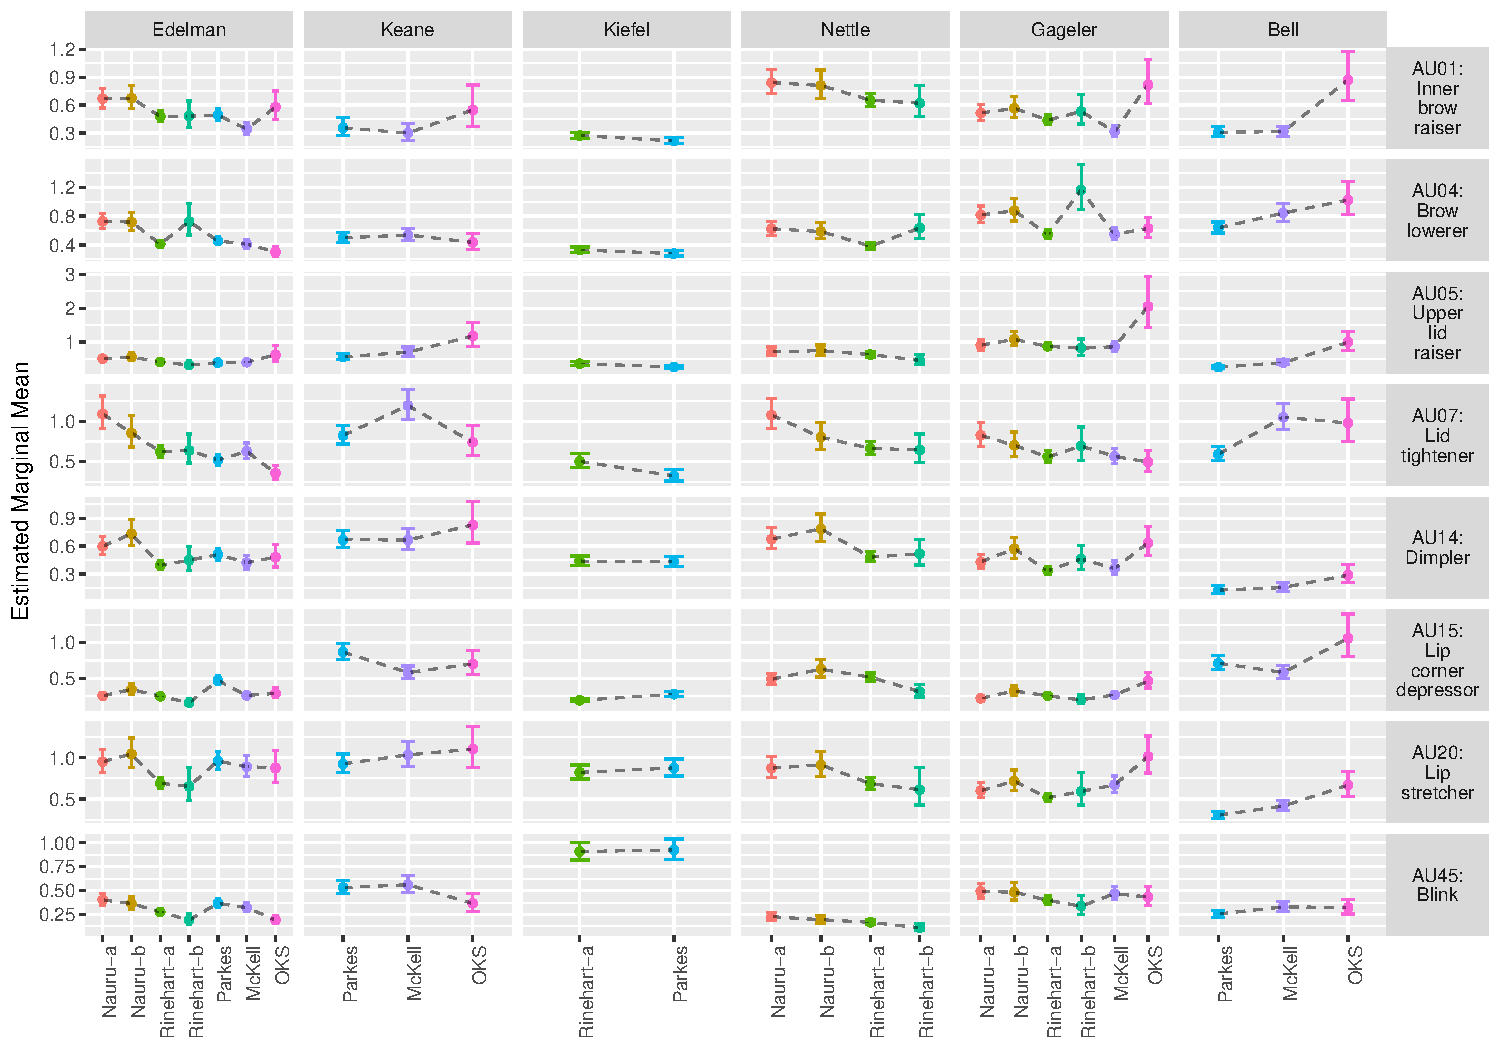
\includegraphics[width=1\linewidth]{figures/intensity-video-1} 

}

\caption{The confidence interval for estimated mearginal mean in model 2}\label{fig:intensity-video}
\end{figure}

\hypertarget{discussion}{%
\section{Discussion}\label{discussion}}

\hypertarget{the-expression-of-the-justices-by-video}{%
\subsection{The expression of the justices by video}\label{the-expression-of-the-justices-by-video}}

Many information can be observed from Figure \ref{fig:model2-plot} for presence and Figure \ref{fig:intensity-video}. The discussion of the two plots will be focusing on answering the question: \textbf{For the same judge, whether the mean presence and mean intensity of the action units are the same or different for different videos}.

In general, we can see that facial expression of the justices are impartial as most of the 95\% confidence intervals for the same judge and action unit overlaps in most of the videos in both plots. While at the same time, there are some time when in a particular video, a judge expressed significantly more or less of an expression and I will break it down to discuss them in more detail.

We can observe that Judge Edelman and Keane behave relatively consistent throughout all the videos since most of the intervals overlap with each other after the bonferroni adjustment. However, Edelman seems to express significantly less in action unit 5 in case OKS. In terms of intensity, Edelman has significantly stronger expression in case Nauru-a, Nauru-b and Rinehart-a in action unit 4 and 9, but more relaxed expression in action unit 7 for case OKS.

To be able to draw some conclusion about the facial behaviour of the Justices, it is necessary to have an understanding about the characteristics of the cases. Nauru-a and Nauru-b discuss the refugee status of the appellants, which can be though of political cases. McKell and OKS are more criminal cases, relates to drug and sexual misconduct. Parkes is a civil case about negligence while Rinehart-a and Rinehart-b are business cases. Based the nature of the 7 cases, we can see Edelman is more likely to express stronger emotion to the political and commercial cases and express less and softer at criminal cases.

For Keane, he appears significantly less action unit 5 in case OKS as Edelman in Figure \ref{fig:model2-plot} but Figure \ref{fig:intensity-video} suggest he has more intense of expression in the same action unit 5. Keane has also more intense expression of action unit 7 in case McKell. This would show that in general Keane is more responsive to the criminal cases than cases of other categories.

Kiefel and Nettle are relatively consistent in their expressions. The presence plot shows that Nettle has relatively higher mean in case Rinehart-b, but it is not significant when comparing the 95\% confidence interval.

Gageler shows a consistent responsive expression in case OKS. In Figure \ref{fig:model2-plot}, Gageler had significantly more expression of action unit 1, 15 and 20. From the intensity plot in Figure \ref{fig:intensity-video}, action unit 5 and 20 have significantly higher intensity. The common associated emotion of action unit 5, 15 and 20 is anger, sad and fear in the six universal emotions. Thus, we can see that Gageler tends to react negatively and more strongly to criminal cases.

Bell also shows a significantly higher proportion of negative emotions associated with action unit 1 and 15 in case OKS and the intensity of action unit 1, 5, 14 and 20 are also significantly higher in case OKS. These evidence indicate the same emotion pattern as judge Gageler to criminal cases. While at the same time, Bell is less reactive in the presence of action unit 07 and 20 in case Parkes and this shows that she has less negative emotion of anger and fear in Parkes, which is the only civil case in our sample videos.

\hypertarget{the-expression-of-the-justices-by-speaker}{%
\subsection{The expression of the justices by speaker}\label{the-expression-of-the-justices-by-speaker}}

From the presence and intensity plot by speakers in Figure \ref{fig:model3-plot} and \ref{fig:intensity-speaker}, we can observe that the video-wise difference between judge are still persist when the speaker effects are included in the model. However, the speaker-wise difference is not significant in terms of both presence and intensity for all the judges.

This result would be a validation that on the high court level, the judges are behaving impartial to different speaking parties.

\hypertarget{summary-1}{%
\section{Summary}\label{summary-1}}

To summarise, the above discussion of intensity and presence of action unit in different cases gives us several findings about the expression of the judges:

\begin{enumerate}
\def\labelenumi{\arabic{enumi})}
\item
  In general, the expression of the Justices are impartial, which is live up to the code of conduct from \textcite{judicalguid} and validate the result from \textcite{tutton2018judicial}.
\item
  When there is significantly present or intense expression of the Justices, it tends to be associated with negative emotion like sad, fear and anger. This could have implication on the mental well-being of the judges.
\item
  Some justices, for example Keane, Gageler and Bell are more responsive, both in frequency (mean presence) and magnitude (mean intensity) to criminal cases. This could show that it is harder for judges to keep a still face when the content of a case goes against human nature.
\end{enumerate}

\hypertarget{conclusion}{%
\chapter{Conclusion}\label{conclusion}}

In this thesis {[}\ldots{}{]}. The cross-sectional data set constructed for each election provides a foundation for statistical modelling of electoral voting behaviour over time. This data will contribute to

The main aim of this research is to {[}\ldots{}{]}. Our approach involves {[}\ldots{}{]}. {[}the more detailed process for getting the data{]}

modelling presence and intensity and summary some results

Our findings {[}\ldots{} link to contribution{]}. Furthermore, as far as we know, this study is the first to {[}\ldots{}{]}. It also provides a workflow for\ldots{}

\hypertarget{limitation}{%
\section{Limitation}\label{limitation}}

I will now briefly discuss some of the limitation of this work. The current image frames are extracted at every one minute interval. However, some facial expressions may only last for a few second. Thus more frequent time interval could be used for getting more precise facial information of the judges. Also, if videos of the high court hearing could be accepted as input for facial expression detection, the potential correlation of emotion could be captured even better.

In my work, seven videos are being processed into the facial recognition software and more videos could be processed to get more robust results. The reason for not processing more videos in the current study is because the resolution of publicly available videos from the high court has only 720 pixels while the facial recognition software, OpenFace requires at least 30 pixels for a face to be detected. This means that we have to choose videos where three or five judges are presented.

However, this work has established a workflow for extracting facial expressions of human from videos. As long as more higher resolution videos are available, facial variables can be extracted via the same fashion.

\hypertarget{future-work}{%
\section{Future work}\label{future-work}}

In the future, more work could be done to extract facial expressions of the Justices from videos using OpenFace. This could enable the researchers to capture more precise expression of the judges. However, as the extraction becomes more frequent, the problem of serial correlation could rise and appropriate modelling technique should be utilised to accommodate for this feature of data.

\hypertarget{acknowledgement}{%
\section{Acknowledgement}\label{acknowledgement}}

The analysis is conducted using R {[}\ref{]}, and the following packages: {[}{]}

\appendix

\hypertarget{appendix}{%
\chapter{Appendix}\label{appendix}}

\hypertarget{list-of-videos-used-in-the-project}{%
\section{List of videos used in the project}\label{list-of-videos-used-in-the-project}}

\begin{longtable}[]{@{}llll@{}}
\caption{Details of videos processed.}\tabularnewline
\toprule
\begin{minipage}[b]{0.22\columnwidth}\raggedright
Case\strut
\end{minipage} & \begin{minipage}[b]{0.15\columnwidth}\raggedright
Name\strut
\end{minipage} & \begin{minipage}[b]{0.30\columnwidth}\raggedright
AV recording link\strut
\end{minipage} & \begin{minipage}[b]{0.22\columnwidth}\raggedright
Judge\strut
\end{minipage}\tabularnewline
\midrule
\endfirsthead
\toprule
\begin{minipage}[b]{0.22\columnwidth}\raggedright
Case\strut
\end{minipage} & \begin{minipage}[b]{0.15\columnwidth}\raggedright
Name\strut
\end{minipage} & \begin{minipage}[b]{0.30\columnwidth}\raggedright
AV recording link\strut
\end{minipage} & \begin{minipage}[b]{0.22\columnwidth}\raggedright
Judge\strut
\end{minipage}\tabularnewline
\midrule
\endhead
\begin{minipage}[t]{0.22\columnwidth}\raggedright
The Republic of Nauru v WET040 {[}No.~2{]} {[}2018{]} HCA 60\strut
\end{minipage} & \begin{minipage}[t]{0.15\columnwidth}\raggedright
\texttt{Nauru\_a}\strut
\end{minipage} & \begin{minipage}[t]{0.30\columnwidth}\raggedright
\url{http://www.hcourt.gov.au/cases/cases-av/av-2018-11-07a}\strut
\end{minipage} & \begin{minipage}[t]{0.22\columnwidth}\raggedright
Nettle, Gageler, Edelman\strut
\end{minipage}\tabularnewline
\begin{minipage}[t]{0.22\columnwidth}\raggedright
TTY167 v Republic of Nauru {[}2018{]} HCA 61\strut
\end{minipage} & \begin{minipage}[t]{0.15\columnwidth}\raggedright
\texttt{Nauru\_b}\strut
\end{minipage} & \begin{minipage}[t]{0.30\columnwidth}\raggedright
\url{http://www.hcourt.gov.au/cases/cases-av/av-2018-11-07b}\strut
\end{minipage} & \begin{minipage}[t]{0.22\columnwidth}\raggedright
Nettle, Gageler, Edelman\strut
\end{minipage}\tabularnewline
\begin{minipage}[t]{0.22\columnwidth}\raggedright
Rinehart v Hancock Prospecting Pty Ltd {[}2019{]} HCA 13\strut
\end{minipage} & \begin{minipage}[t]{0.15\columnwidth}\raggedright
\texttt{Rinehart\_a}\strut
\end{minipage} & \begin{minipage}[t]{0.30\columnwidth}\raggedright
\url{http://www.hcourt.gov.au/cases/cases-av/av-2018-11-13}\strut
\end{minipage} & \begin{minipage}[t]{0.22\columnwidth}\raggedright
Gordon, Gageler, Bell, Keane, Edelman\strut
\end{minipage}\tabularnewline
\begin{minipage}[t]{0.22\columnwidth}\raggedright
Rinehart v Hancock Prospecting Pty Ltd {[}2019{]} HCA 13\strut
\end{minipage} & \begin{minipage}[t]{0.15\columnwidth}\raggedright
\texttt{Rinehart\_b}\strut
\end{minipage} & \begin{minipage}[t]{0.30\columnwidth}\raggedright
\url{http://www.hcourt.gov.au/cases/cases-av/av-2018-11-14a}\strut
\end{minipage} & \begin{minipage}[t]{0.22\columnwidth}\raggedright
Gordon, Keane, Bell, Gageler, Edelman\strut
\end{minipage}\tabularnewline
\begin{minipage}[t]{0.22\columnwidth}\raggedright
Parkes Shire Council v South West Helicopters Pty Limited {[}2019{]} HCA 14\strut
\end{minipage} & \begin{minipage}[t]{0.15\columnwidth}\raggedright
\texttt{Parkes}\strut
\end{minipage} & \begin{minipage}[t]{0.30\columnwidth}\raggedright
\url{http://www.hcourt.gov.au/cases/cases-av/av-2018-11-14b}\strut
\end{minipage} & \begin{minipage}[t]{0.22\columnwidth}\raggedright
Gordon, Bell, Kiefel, Keane, Edelman\strut
\end{minipage}\tabularnewline
\begin{minipage}[t]{0.22\columnwidth}\raggedright
McKell v The Queen {[}2019{]} HCA 5\strut
\end{minipage} & \begin{minipage}[t]{0.15\columnwidth}\raggedright
\texttt{McKell}\strut
\end{minipage} & \begin{minipage}[t]{0.30\columnwidth}\raggedright
\url{http://www.hcourt.gov.au/cases/cases-av/av-2018-12-07}\strut
\end{minipage} & \begin{minipage}[t]{0.22\columnwidth}\raggedright
Gordon, Gageler, Kiefel, Nettle, Edelman\strut
\end{minipage}\tabularnewline
\begin{minipage}[t]{0.22\columnwidth}\raggedright
OKS v Western Australia {[}2019{]} HCA 10\strut
\end{minipage} & \begin{minipage}[t]{0.15\columnwidth}\raggedright
\texttt{OKS}\strut
\end{minipage} & \begin{minipage}[t]{0.30\columnwidth}\raggedright
\url{http://www.hcourt.gov.au/cases/cases-av/av-2019-02-14}\strut
\end{minipage} & \begin{minipage}[t]{0.22\columnwidth}\raggedright
Gordon, Gageler, Kiefel, Nettle, Edelman\strut
\end{minipage}\tabularnewline
\bottomrule
\end{longtable}

\hypertarget{model-estimation-result}{%
\section{Model estimation result}\label{model-estimation-result}}

\begin{center}
\begin{longtable}{lllllll}
\caption{\label{tab:result-2}model result 2 for mean presence}\\
\toprule
judge & video & AU & prob & SE & asymp.LCL & asymp.UCL \\
\midrule
\endhead
\bottomrule
\endfoot
Edelman & Nauru-a & AU01 & 0.678 & 0.0276 & 0.599 & 0.747 \\
Nettle & Nauru-a & AU01 & 0.721 & 0.0269 & 0.643 & 0.787 \\
Gageler & Nauru-a & AU01 & 0.337 & 0.0283 & 0.265 & 0.417 \\
Edelman & Nauru-b & AU01 & 0.589 & 0.0354 & 0.491 & 0.680 \\
Nettle & Nauru-b & AU01 & 0.673 & 0.0337 & 0.577 & 0.756 \\
Gageler & Nauru-b & AU01 & 0.273 & 0.0302 & 0.200 & 0.362 \\
Edelman & Rinehart-a & AU01 & 0.597 & 0.0212 & 0.539 & 0.652 \\
Kiefel & Rinehart-a & AU01 & 0.524 & 0.0245 & 0.458 & 0.589 \\
Nettle & Rinehart-a & AU01 & 0.698 & 0.0215 & 0.637 & 0.752 \\
Gageler & Rinehart-a & AU01 & 0.324 & 0.0208 & 0.270 & 0.382 \\
Edelman & Rinehart-b & AU01 & 0.628 & 0.0561 & 0.469 & 0.763 \\
Nettle & Rinehart-b & AU01 & 0.824 & 0.0376 & 0.700 & 0.904 \\
Gageler & Rinehart-b & AU01 & 0.409 & 0.0577 & 0.267 & 0.569 \\
Edelman & McKell & AU01 & 0.419 & 0.0316 & 0.337 & 0.506 \\
Keane & McKell & AU01 & 0.054 & 0.0107 & 0.031 & 0.091 \\
Gageler & McKell & AU01 & 0.248 & 0.0264 & 0.184 & 0.326 \\
Bell & McKell & AU01 & 0.650 & 0.0330 & 0.557 & 0.733 \\
Edelman & OKS & AU01 & 0.564 & 0.0546 & 0.415 & 0.701 \\
Keane & OKS & AU01 & 0.220 & 0.0436 & 0.124 & 0.358 \\
Gageler & OKS & AU01 & 0.586 & 0.0535 & 0.439 & 0.719 \\
Bell & OKS & AU01 & 0.940 & 0.0156 & 0.882 & 0.970 \\
Edelman & Parkes & AU01 & 0.606 & 0.0255 & 0.535 & 0.672 \\
Keane & Parkes & AU01 & 0.122 & 0.0185 & 0.080 & 0.181 \\
Kiefel & Parkes & AU01 & 0.446 & 0.0277 & 0.373 & 0.521 \\
Bell & Parkes & AU01 & 0.673 & 0.0273 & 0.596 & 0.742 \\
Edelman & Nauru-a & AU04 & 0.573 & 0.0298 & 0.492 & 0.651 \\
Nettle & Nauru-a & AU04 & 0.386 & 0.0302 & 0.309 & 0.470 \\
Gageler & Nauru-a & AU04 & 0.471 & 0.0303 & 0.391 & 0.553 \\
Edelman & Nauru-b & AU04 & 0.535 & 0.0356 & 0.439 & 0.628 \\
Nettle & Nauru-b & AU04 & 0.387 & 0.0353 & 0.297 & 0.485 \\
Gageler & Nauru-b & AU04 & 0.454 & 0.0355 & 0.361 & 0.550 \\
Edelman & Rinehart-a & AU04 & 0.314 & 0.0202 & 0.263 & 0.371 \\
Kiefel & Rinehart-a & AU04 & 0.082 & 0.0122 & 0.055 & 0.121 \\
Nettle & Rinehart-a & AU04 & 0.215 & 0.0184 & 0.169 & 0.268 \\
Gageler & Rinehart-a & AU04 & 0.290 & 0.0199 & 0.239 & 0.346 \\
Edelman & Rinehart-b & AU04 & 0.466 & 0.0567 & 0.321 & 0.617 \\
Nettle & Rinehart-b & AU04 & 0.481 & 0.0578 & 0.332 & 0.634 \\
Gageler & Rinehart-b & AU04 & 0.497 & 0.0567 & 0.349 & 0.645 \\
Edelman & McKell & AU04 & 0.352 & 0.0291 & 0.279 & 0.434 \\
Keane & McKell & AU04 & 0.176 & 0.0233 & 0.121 & 0.248 \\
Gageler & McKell & AU04 & 0.406 & 0.0319 & 0.324 & 0.493 \\
Bell & McKell & AU04 & 0.672 & 0.0315 & 0.583 & 0.751 \\
Edelman & OKS & AU04 & 0.176 & 0.0346 & 0.101 & 0.289 \\
Keane & OKS & AU04 & 0.189 & 0.0378 & 0.107 & 0.311 \\
Gageler & OKS & AU04 & 0.392 & 0.0527 & 0.262 & 0.539 \\
Bell & OKS & AU04 & 0.791 & 0.0406 & 0.662 & 0.880 \\
Edelman & Parkes & AU04 & 0.460 & 0.0273 & 0.388 & 0.533 \\
Keane & Parkes & AU04 & 0.277 & 0.0259 & 0.213 & 0.352 \\
Kiefel & Parkes & AU04 & 0.105 & 0.0156 & 0.069 & 0.155 \\
Bell & Parkes & AU04 & 0.626 & 0.0280 & 0.548 & 0.697 \\
Edelman & Nauru-a & AU05 & 0.323 & 0.0280 & 0.252 & 0.402 \\
Nettle & Nauru-a & AU05 & 0.215 & 0.0237 & 0.158 & 0.286 \\
Gageler & Nauru-a & AU05 & 0.628 & 0.0296 & 0.545 & 0.703 \\
Edelman & Nauru-b & AU05 & 0.284 & 0.0313 & 0.208 & 0.375 \\
Nettle & Nauru-b & AU05 & 0.211 & 0.0273 & 0.146 & 0.294 \\
Gageler & Nauru-b & AU05 & 0.604 & 0.0358 & 0.505 & 0.696 \\
Edelman & Rinehart-a & AU05 & 0.333 & 0.0204 & 0.280 & 0.390 \\
Kiefel & Rinehart-a & AU05 & 0.391 & 0.0240 & 0.328 & 0.457 \\
Nettle & Rinehart-a & AU05 & 0.267 & 0.0207 & 0.215 & 0.326 \\
Gageler & Rinehart-a & AU05 & 0.702 & 0.0202 & 0.645 & 0.754 \\
Edelman & Rinehart-b & AU05 & 0.218 & 0.0430 & 0.124 & 0.355 \\
Nettle & Rinehart-b & AU05 & 0.266 & 0.0493 & 0.155 & 0.417 \\
Gageler & Rinehart-b & AU05 & 0.627 & 0.0567 & 0.467 & 0.763 \\
Edelman & McKell & AU05 & 0.289 & 0.0269 & 0.222 & 0.366 \\
Keane & McKell & AU05 & 0.537 & 0.0341 & 0.445 & 0.626 \\
Gageler & McKell & AU05 & 0.731 & 0.0271 & 0.652 & 0.797 \\
Bell & McKell & AU05 & 0.648 & 0.0317 & 0.559 & 0.728 \\
Edelman & OKS & AU05 & 0.053 & 0.0129 & 0.027 & 0.101 \\
Keane & OKS & AU05 & 0.308 & 0.0490 & 0.194 & 0.452 \\
Gageler & OKS & AU05 & 0.475 & 0.0548 & 0.334 & 0.620 \\
Bell & OKS & AU05 & 0.545 & 0.0560 & 0.395 & 0.687 \\
Edelman & Parkes & AU05 & 0.295 & 0.0231 & 0.237 & 0.360 \\
Keane & Parkes & AU05 & 0.578 & 0.0284 & 0.500 & 0.652 \\
Kiefel & Parkes & AU05 & 0.275 & 0.0240 & 0.215 & 0.344 \\
Bell & Parkes & AU05 & 0.496 & 0.0289 & 0.419 & 0.573 \\
Edelman & Nauru-a & AU07 & 0.439 & 0.0301 & 0.361 & 0.521 \\
Nettle & Nauru-a & AU07 & 0.511 & 0.0312 & 0.427 & 0.593 \\
Gageler & Nauru-a & AU07 & 0.269 & 0.0253 & 0.206 & 0.342 \\
Edelman & Nauru-b & AU07 & 0.402 & 0.0350 & 0.312 & 0.498 \\
Nettle & Nauru-b & AU07 & 0.511 & 0.0368 & 0.413 & 0.609 \\
Gageler & Nauru-b & AU07 & 0.255 & 0.0290 & 0.185 & 0.341 \\
Edelman & Rinehart-a & AU07 & 0.378 & 0.0212 & 0.323 & 0.437 \\
Kiefel & Rinehart-a & AU07 & 0.175 & 0.0182 & 0.132 & 0.230 \\
Nettle & Rinehart-a & AU07 & 0.507 & 0.0237 & 0.443 & 0.570 \\
Gageler & Rinehart-a & AU07 & 0.277 & 0.0195 & 0.227 & 0.332 \\
Edelman & Rinehart-b & AU07 & 0.316 & 0.0517 & 0.195 & 0.468 \\
Nettle & Rinehart-b & AU07 & 0.582 & 0.0579 & 0.423 & 0.725 \\
Gageler & Rinehart-b & AU07 & 0.269 & 0.0476 & 0.161 & 0.414 \\
Edelman & McKell & AU07 & 0.422 & 0.0304 & 0.343 & 0.505 \\
Keane & McKell & AU07 & 0.646 & 0.0321 & 0.555 & 0.727 \\
Gageler & McKell & AU07 & 0.393 & 0.0314 & 0.312 & 0.480 \\
Bell & McKell & AU07 & 0.714 & 0.0294 & 0.629 & 0.786 \\
Edelman & OKS & AU07 & 0.246 & 0.0422 & 0.150 & 0.376 \\
Keane & OKS & AU07 & 0.694 & 0.0485 & 0.550 & 0.807 \\
Gageler & OKS & AU07 & 0.411 & 0.0522 & 0.281 & 0.554 \\
Bell & OKS & AU07 & 0.840 & 0.0334 & 0.729 & 0.911 \\
Edelman & Parkes & AU07 & 0.380 & 0.0257 & 0.313 & 0.451 \\
Keane & Parkes & AU07 & 0.637 & 0.0276 & 0.560 & 0.708 \\
Kiefel & Parkes & AU07 & 0.131 & 0.0167 & 0.092 & 0.183 \\
Bell & Parkes & AU07 & 0.522 & 0.0291 & 0.444 & 0.599 \\
Edelman & Nauru-a & AU14 & 0.465 & 0.0299 & 0.386 & 0.545 \\
Nettle & Nauru-a & AU14 & 0.465 & 0.0307 & 0.384 & 0.548 \\
Gageler & Nauru-a & AU14 & 0.567 & 0.0297 & 0.486 & 0.644 \\
Edelman & Nauru-b & AU14 & 0.477 & 0.0354 & 0.384 & 0.572 \\
Nettle & Nauru-b & AU14 & 0.517 & 0.0363 & 0.420 & 0.613 \\
Gageler & Nauru-b & AU14 & 0.600 & 0.0344 & 0.505 & 0.688 \\
Edelman & Rinehart-a & AU14 & 0.404 & 0.0210 & 0.349 & 0.462 \\
Kiefel & Rinehart-a & AU14 & 0.552 & 0.0243 & 0.486 & 0.616 \\
Nettle & Rinehart-a & AU14 & 0.463 & 0.0235 & 0.401 & 0.527 \\
Gageler & Rinehart-a & AU14 & 0.578 & 0.0221 & 0.517 & 0.636 \\
Edelman & Rinehart-b & AU14 & 0.491 & 0.0582 & 0.340 & 0.643 \\
Nettle & Rinehart-b & AU14 & 0.686 & 0.0519 & 0.533 & 0.807 \\
Gageler & Rinehart-b & AU14 & 0.712 & 0.0489 & 0.566 & 0.825 \\
Edelman & McKell & AU14 & 0.448 & 0.0313 & 0.366 & 0.533 \\
Keane & McKell & AU14 & 0.697 & 0.0310 & 0.608 & 0.773 \\
Gageler & McKell & AU14 & 0.699 & 0.0285 & 0.617 & 0.770 \\
Bell & McKell & AU14 & 0.179 & 0.0251 & 0.121 & 0.257 \\
Edelman & OKS & AU14 & 0.352 & 0.0507 & 0.230 & 0.497 \\
Keane & OKS & AU14 & 0.810 & 0.0372 & 0.690 & 0.891 \\
Gageler & OKS & AU14 & 0.789 & 0.0379 & 0.669 & 0.873 \\
Bell & OKS & AU14 & 0.406 & 0.0560 & 0.268 & 0.561 \\
Edelman & Parkes & AU14 & 0.414 & 0.0257 & 0.347 & 0.484 \\
Keane & Parkes & AU14 & 0.696 & 0.0264 & 0.621 & 0.762 \\
Kiefel & Parkes & AU14 & 0.475 & 0.0278 & 0.401 & 0.549 \\
Bell & Parkes & AU14 & 0.090 & 0.0139 & 0.058 & 0.135 \\
Edelman & Nauru-a & AU15 & 0.377 & 0.0290 & 0.303 & 0.458 \\
Nettle & Nauru-a & AU15 & 0.699 & 0.0280 & 0.619 & 0.769 \\
Gageler & Nauru-a & AU15 & 0.480 & 0.0306 & 0.399 & 0.562 \\
Edelman & Nauru-b & AU15 & 0.503 & 0.0367 & 0.406 & 0.601 \\
Nettle & Nauru-b & AU15 & 0.820 & 0.0247 & 0.744 & 0.877 \\
Gageler & Nauru-b & AU15 & 0.627 & 0.0348 & 0.530 & 0.715 \\
Edelman & Rinehart-a & AU15 & 0.457 & 0.0217 & 0.399 & 0.516 \\
Kiefel & Rinehart-a & AU15 & 0.454 & 0.0244 & 0.389 & 0.520 \\
Nettle & Rinehart-a & AU15 & 0.804 & 0.0179 & 0.751 & 0.847 \\
Gageler & Rinehart-a & AU15 & 0.632 & 0.0217 & 0.572 & 0.688 \\
Edelman & Rinehart-b & AU15 & 0.318 & 0.0525 & 0.195 & 0.472 \\
Nettle & Rinehart-b & AU15 & 0.802 & 0.0409 & 0.669 & 0.890 \\
Gageler & Rinehart-b & AU15 & 0.547 & 0.0588 & 0.390 & 0.696 \\
Edelman & McKell & AU15 & 0.443 & 0.0318 & 0.360 & 0.530 \\
Keane & McKell & AU15 & 0.823 & 0.0253 & 0.744 & 0.881 \\
Gageler & McKell & AU15 & 0.697 & 0.0291 & 0.613 & 0.769 \\
Bell & McKell & AU15 & 0.871 & 0.0203 & 0.806 & 0.917 \\
Edelman & OKS & AU15 & 0.497 & 0.0618 & 0.337 & 0.657 \\
Keane & OKS & AU15 & 0.941 & 0.0175 & 0.872 & 0.974 \\
Gageler & OKS & AU15 & 0.873 & 0.0306 & 0.766 & 0.935 \\
Bell & OKS & AU15 & 0.975 & 0.0080 & 0.942 & 0.990 \\
Edelman & Parkes & AU15 & 0.514 & 0.0266 & 0.443 & 0.585 \\
Keane & Parkes & AU15 & 0.876 & 0.0178 & 0.820 & 0.917 \\
Kiefel & Parkes & AU15 & 0.424 & 0.0275 & 0.353 & 0.499 \\
Bell & Parkes & AU15 & 0.824 & 0.0220 & 0.757 & 0.876 \\
Edelman & Nauru-a & AU20 & 0.780 & 0.0233 & 0.711 & 0.836 \\
Nettle & Nauru-a & AU20 & 0.727 & 0.0269 & 0.649 & 0.793 \\
Gageler & Nauru-a & AU20 & 0.467 & 0.0311 & 0.385 & 0.551 \\
Edelman & Nauru-b & AU20 & 0.767 & 0.0282 & 0.683 & 0.834 \\
Nettle & Nauru-b & AU20 & 0.743 & 0.0305 & 0.653 & 0.817 \\
Gageler & Nauru-b & AU20 & 0.470 & 0.0369 & 0.373 & 0.569 \\
Edelman & Rinehart-a & AU20 & 0.754 & 0.0183 & 0.701 & 0.800 \\
Kiefel & Rinehart-a & AU20 & 0.868 & 0.0156 & 0.820 & 0.905 \\
Nettle & Rinehart-a & AU20 & 0.745 & 0.0202 & 0.687 & 0.796 \\
Gageler & Rinehart-a & AU20 & 0.503 & 0.0230 & 0.442 & 0.565 \\
Edelman & Rinehart-b & AU20 & 0.664 & 0.0536 & 0.509 & 0.790 \\
Nettle & Rinehart-b & AU20 & 0.771 & 0.0444 & 0.631 & 0.869 \\
Gageler & Rinehart-b & AU20 & 0.454 & 0.0583 & 0.306 & 0.611 \\
Edelman & McKell & AU20 & 0.838 & 0.0205 & 0.775 & 0.886 \\
Keane & McKell & AU20 & 0.952 & 0.0113 & 0.911 & 0.975 \\
Gageler & McKell & AU20 & 0.707 & 0.0302 & 0.620 & 0.782 \\
Bell & McKell & AU20 & 0.768 & 0.0285 & 0.683 & 0.835 \\
Edelman & OKS & AU20 & 0.898 & 0.0320 & 0.775 & 0.958 \\
Keane & OKS & AU20 & 0.990 & 0.0045 & 0.967 & 0.997 \\
Gageler & OKS & AU20 & 0.909 & 0.0292 & 0.794 & 0.963 \\
Bell & OKS & AU20 & 0.964 & 0.0135 & 0.904 & 0.987 \\
Edelman & Parkes & AU20 & 0.732 & 0.0238 & 0.664 & 0.791 \\
Keane & Parkes & AU20 & 0.924 & 0.0153 & 0.871 & 0.956 \\
Kiefel & Parkes & AU20 & 0.806 & 0.0217 & 0.740 & 0.857 \\
Bell & Parkes & AU20 & 0.477 & 0.0302 & 0.397 & 0.558 \\
Edelman & Nauru-a & AU45 & 0.200 & 0.0238 & 0.144 & 0.272 \\
Nettle & Nauru-a & AU45 & 0.091 & 0.0157 & 0.056 & 0.143 \\
Gageler & Nauru-a & AU45 & 0.384 & 0.0319 & 0.303 & 0.473 \\
Edelman & Nauru-b & AU45 & 0.136 & 0.0224 & 0.087 & 0.209 \\
Nettle & Nauru-b & AU45 & 0.069 & 0.0144 & 0.039 & 0.119 \\
Gageler & Nauru-b & AU45 & 0.300 & 0.0362 & 0.212 & 0.405 \\
Edelman & Rinehart-a & AU45 & 0.124 & 0.0131 & 0.093 & 0.164 \\
Kiefel & Rinehart-a & AU45 & 0.825 & 0.0185 & 0.770 & 0.869 \\
Nettle & Rinehart-a & AU45 & 0.067 & 0.0106 & 0.043 & 0.102 \\
Gageler & Rinehart-a & AU45 & 0.321 & 0.0220 & 0.265 & 0.383 \\
Edelman & Rinehart-b & AU45 & 0.067 & 0.0215 & 0.028 & 0.154 \\
Nettle & Rinehart-b & AU45 & 0.061 & 0.0206 & 0.024 & 0.146 \\
Gageler & Rinehart-b & AU45 & 0.233 & 0.0564 & 0.115 & 0.415 \\
Edelman & McKell & AU45 & 0.114 & 0.0157 & 0.078 & 0.164 \\
Keane & McKell & AU45 & 0.540 & 0.0353 & 0.445 & 0.633 \\
Gageler & McKell & AU45 & 0.378 & 0.0330 & 0.294 & 0.470 \\
Bell & McKell & AU45 & 0.180 & 0.0244 & 0.123 & 0.255 \\
Edelman & OKS & AU45 & 0.023 & 0.0065 & 0.011 & 0.048 \\
Keane & OKS & AU45 & 0.372 & 0.0562 & 0.237 & 0.531 \\
Gageler & OKS & AU45 & 0.209 & 0.0420 & 0.118 & 0.344 \\
Bell & OKS & AU45 & 0.158 & 0.0359 & 0.083 & 0.279 \\
Edelman & Parkes & AU45 & 0.226 & 0.0221 & 0.172 & 0.291 \\
Keane & Parkes & AU45 & 0.754 & 0.0243 & 0.682 & 0.813 \\
Kiefel & Parkes & AU45 & 0.872 & 0.0170 & 0.819 & 0.912 \\
Bell & Parkes & AU45 & 0.205 & 0.0230 & 0.150 & 0.274 \\
\end{longtable}
\end{center}

\begin{figure}

{\centering 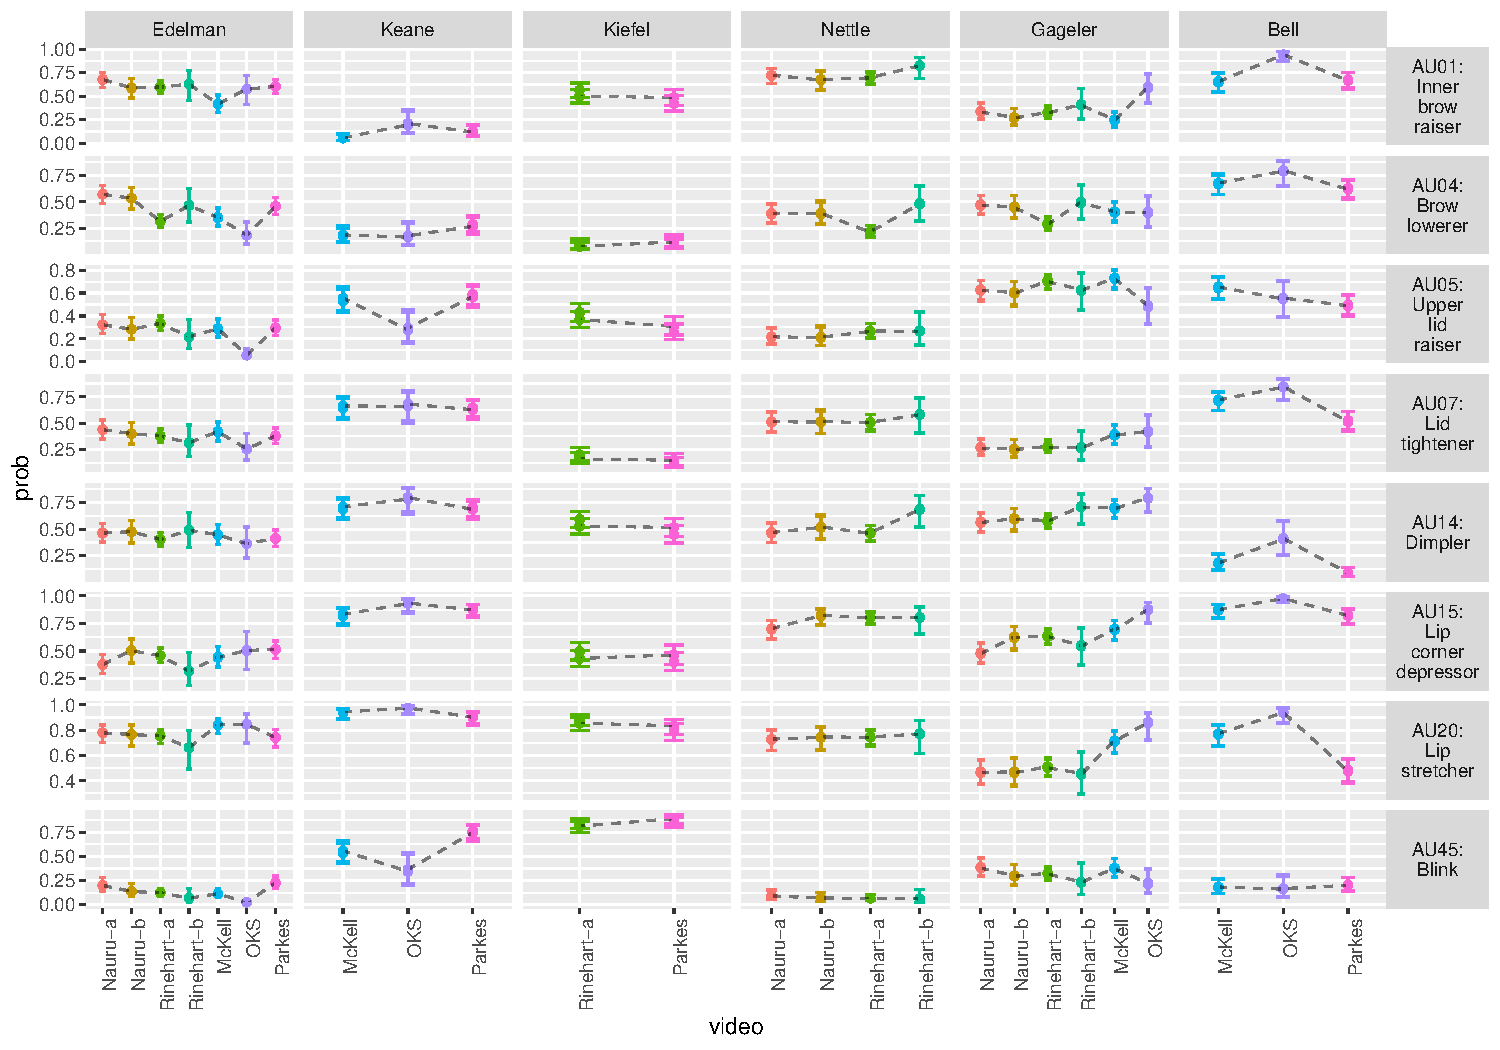
\includegraphics[width=1\linewidth]{figures/model3-plot-1} 

}

\caption{The confidence interval for estimated mearginal mean in model 3}\label{fig:model3-plot}
\end{figure}

\begin{figure}

{\centering 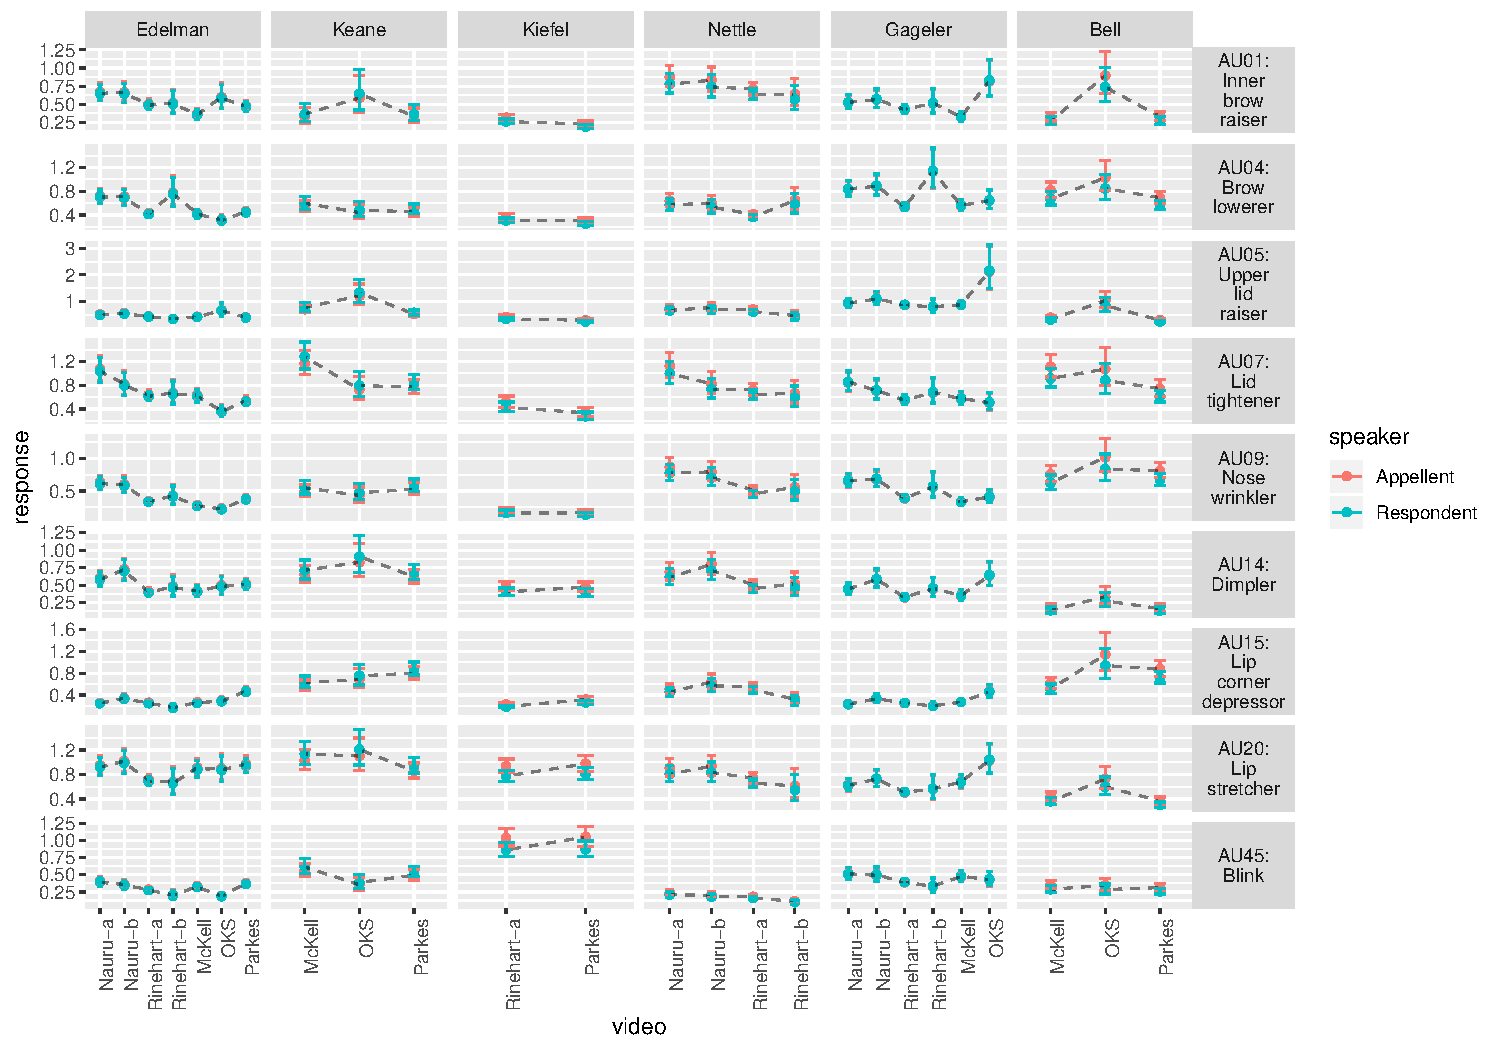
\includegraphics[width=1\linewidth]{figures/intensity-speaker-1} 

}

\caption{The confidence interval for estimated mearginal mean in model 3}\label{fig:intensity-speaker}
\end{figure}

\printbibliography[heading=bibintoc]



\end{document}
